\documentclass{article}
\usepackage{graphicx}
\DeclareGraphicsExtensions{.pdf}

\usepackage[final]{pdfpages}

\headheight 0in
\oddsidemargin 0in
\evensidemargin  0in
\topmargin  -.25in
\textwidth 6.5in
\textheight 9in
\title{OMPT: An OpenMP\textsuperscript{\textregistered} Tools Application Programming Interface for Performance Analysis}
\author{Alexandre Eichenberger\thanks{IBM T.J. Watson Research Center}, 
John Mellor-Crummey\thanks{Rice University}, 
Martin Schulz\thanks{Lawrence Livermore National Laboratory},
\\~\\
Nawal Copty\thanks{Oracle}, 
Jim Cownie\thanks{Intel},
Tim Cramer\thanks{RWTH Aachen University}, 
Robert Dietrich\thanks{TU Dresden, ZIH},
Xu Liu\hbox to 0in{$^\dagger$\hss},
Eugene Loh\hbox to 0in{$^\S$\hss}, 
Daniel Lorenz\thanks{J\"{u}lich Supercomputer Center}, 
\\
and other members of the OpenMP Tools Working Group}
\date{Revised June 22, 2016}

\usepackage{comment}
\usepackage{needspace}
\usepackage[colorlinks=true,citecolor=blue]{hyper ref}
\usepackage{url}
\usepackage{xcolor}
\RequirePackage[normalem]{ulem} 

\usepackage{listings}
\lstdefinelanguage{diff}{
%   morecomment=[f][\color{red!80!black}]-,         % deleted lines 
%   morecomment=[f][\color{green!60!black}]+,       % added lines
%   moredelim=[is][\color{red!80!black}]{-*}{*-},
%   moredelim=[is][\color{green!60!black}]{+*}{*+},
  morecomment=[f][\color{red}\sout]-,         % deleted lines 
  morecomment=[f][\color{blue}\uwave]+,       % added lines
  moredelim=[is][\color{red}\sout]{-*-}{-*-},
  moredelim=[is][\color{blue}\uwave]{+*+}{+*+},
}
\lstdefinestyle{cstyle}{
  belowcaptionskip=.25\baselineskip,
  language=diff,
  showstringspaces=false,
  basicstyle=\ttfamily,
  keywordstyle=\bfseries\color{green!60!black},
  commentstyle=\itshape\color{purple!40!black},
  columns=fullflexible,
  keepspaces=true,
  float,
  floatplacement=H,
  belowskip=\smallskipamount,
  aboveskip=\smallskipamount,
%   belowskip=-\baselineskip,
}
\lstset{style=cstyle}

\newcommand{\descheader}[1]{{\needspace{3\baselineskip}\vspace{1em}\noindent \fbox{#1}}}


\begin{document}  
\begin{comment}   
\pagestyle{empty}
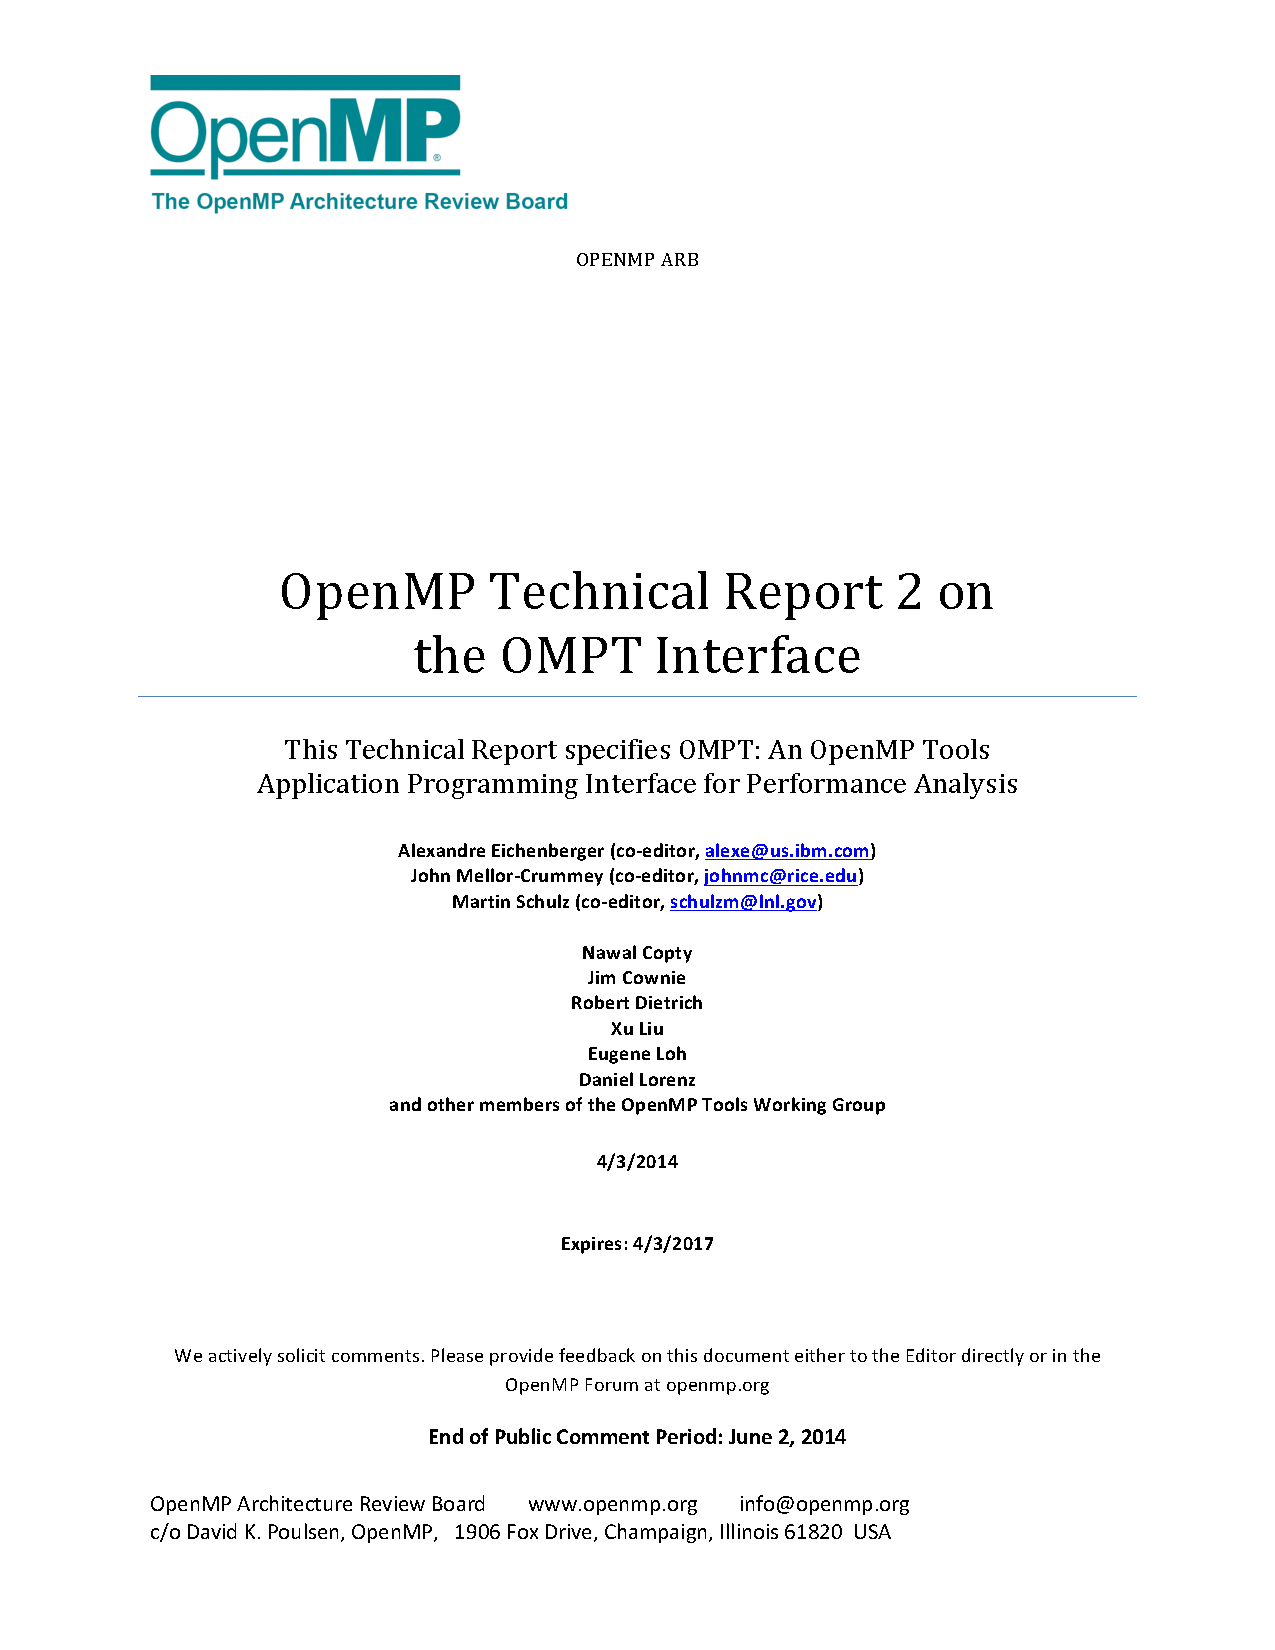
\includepdf[
   pages={-},
   pagecommand={},
 ]{OMPT_TR_header}
 
\setcounter{page}{1}
\pagestyle{plain}
\end{comment}
                                           
\maketitle
\section{Introduction}
Today, it is difficult to produce high quality tools that support 
% debugging and/or 
performance analysis of OpenMP programs without tightly integrating them with a specific OpenMP runtime implementation. To address this problem, this document defines OMPT---an application programming interface (API) for first-party performance tools.\footnote{A {\em first-party} tool runs within the address space of an application process. This differs from a {\em third-party} tool, e.g., a debugger, which runs as a separate process.}  
Extending the OpenMP standard with this API  will make it possible to construct powerful tools that will support any standard-compliant OpenMP implementation.

\subsection{OMPT}

The design of OMPT is based on experience with two prior efforts to define a standard OpenMP tools API: the POMP API~\cite{Mohr:EWOMP02} and the Sun/Oracle Collector API~\cite{SunCollector,Jost:2005:AND:1892830.1892858}. 
The POMP API provides support for instrumentation-based measurement. A drawback of this approach  is that its overhead can be significant because an operation, e.g., an iteration of an OpenMP worksharing loop, may take less time than tool callbacks monitoring its execution. 
In contrast, 
the Sun/Oracle Collector API was  designed primarily to support performance measurement 
using asynchronous sampling. This  design enables the construction of tools that attribute costs without the overhead and intrusion of pervasive instrumentation. With the Collector API, tools
 can use low-overhead asynchronous  sampling of application call stacks to record compact call path profiles. However, the Collector API doesn't provide enough instrumentation hooks to provide full tool support for statically-linked executables.
OMPT builds upon ideas from both the POMP and  Collector APIs. The core of OMPT is a minimal set of features to support tools that employ asynchronous sampling to measure application performance. In addition, OMPT defines  interfaces to support  {\em blame shifting}~\cite{Tallent:PPoPP09,Tallent:PPoPP10}---a technique that shifts attribution of costs from symptoms to causes.
Finally, OMPT defines callbacks suitable for instrumentation-based monitoring of runtime events. 
 OMPT can be implemented entirely by a compiler, entirely by an OpenMP runtime system, or with a hybrid strategy that employs a mixture of compiler and runtime support.

With the exception of one routine for tool control, all functions in the OMPT API are intended for use only by tools rather than by applications. All OMPT API functions  have a C binding. A Fortran binding is  provided only for the single application-facing tool control function described in Section~\ref{sec:app-facing}.

In some cases, the OMPT API may enable a tool to infer details and observe performance implications about the implementation chosen by an OpenMP compiler and runtime. An OpenMP implementation may differ from the abstract execution model described by the OpenMP standard. The ability of tools using OMPT  to observe such differences does not affect the language implementation's ability to optimize using the ``as if'' rule described in the OpenMP standard.

\subsubsection{Design Objectives}
OMPT tries to satisfy several design objectives for a performance tool interface for OpenMP. These objectives are listed in decreasing order of importance.
\begin{itemize}
\item The API should allow tools to gather sufficient information about an OpenMP program execution to associate costs with both the program and the OpenMP runtime.
\begin{itemize}
\item The API should provide an interface sufficient to construct low-overhead performance tools based on asynchronous sampling.
\item The API should enable a profiler that uses call stack unwinding to identify which frames in its call stack are present on behalf of the OpenMP runtime.
\item The OpenMP runtime should associate the activity of a thread at any point in time with a {\em state}, e.g., idle, which will enable a performance tool to interpret program behavior.  
\item Certain API routines must be defined as {\em async signal safe} so that they can be invoked in a profiler's signal handler as it processes interrupts generated by asynchronous sampling.
\end{itemize}
\item Incorporating support for the  API in an OpenMP runtime should add negligible overhead to the runtime system if the interface is not in use by a tool.
\item The API should define interfaces suitable for constructing  instrumentation-based performance tools.
\item Adding the API to an OpenMP runtime should not impose an unreasonable development burden on the runtime developer.
\item The API should not impose an unreasonable development burden on tool implementers.
\end{itemize}

To support the OMPT interface for tools, an OpenMP runtime must maintain information about the state of each OpenMP thread and provide a set of API calls that tools can use to interrogate the OpenMP runtime. Maintaining information about the state of each thread in the runtime system is not free and thus an OpenMP runtime need not maintain state information unless a tool has registered its interest in this information.
Without any explicit request to enable tool support, an OpenMP runtime need not maintain any state for the benefit of tools.

\subsubsection{Minimally Compliant Implementation}

OMPT has a small set of mandatory features that provide a common foundation for all performance tools. A runtime may also implement additional, optional, OMPT features used by some tools to gather extra information about a program execution.     
The features required by a minimally compliant implementation are summarized below.

\begin{itemize}
\item Maintain a unique identifier per OpenMP thread, parallel region, task region, target region, and target operation. In addition, each thread maintains a wait identifier.
\item Maintain pointers into the stack for each OpenMP thread to distinguish frames for user procedures from frames for OpenMP runtime routines.  
\item Maintain a state and a wait condition for each OpenMP thread. Mandatory states are idle, work serial, work parallel, and undefined.
\item Provide callbacks to tools when encountering the following  events:  thread begin/end, parallel region begin/end, task create, task schedule, implicit task begin/end, target region begin/end, target data operation, target submission, a user-level tool control call, and runtime shutdown.
\item Implement several async signal safe inquiry functions to retrieve information from the OpenMP runtime.
\item Have the OpenMP runtime initiate a callback to a tool initialization routine 
as directed by the value of a new OpenMP environment variable (\code{OMP\_TOOL}) and provide a function to register tool callbacks with the runtime.
\end{itemize}

\subsection{Document Roadmap}
This document first outlines various aspects of the OMPT tools API. 
Section~\ref{sec:states} describes the state information maintained by the OpenMP runtime on behalf of OMPT for use by tools.
Section~\ref{sec:events} describes the OMPT callbacks to notify a tool of various OpenMP runtime events during an execution.
Section~\ref{sec:data} describes the data structures used by the OMPT interface.
Section~\ref{sec:inquiry} describes the runtime system inquiry operations supported by OMPT for the benefit of tools.
Section~\ref{sec:target-device-records} describes an API for tracing activities on target devices.
Section~\ref{sec:enabling} describes the OMPT API operations for tool initialization.
Section~\ref{sec:app-facing} describes the tool control interface available to applications.
Appendix~\ref{appendix:ompt-types} provides a definition of the complete OMPT interface in C.
Appendix~\ref{app:frame} illustrates the information that OMPT maintains about call stacks and the use of OMPT API routines to inspect it; this support enables tools to associate code executed in OpenMP parallel regions with  application-level calling contexts. 
% Appendix~\ref{app:registration} outlines some considerations that impact the design of the interface for tool registration.

\section{Runtime States} 
\label{sec:states} 

To enable a tool to understand what an OpenMP thread is doing, when a tool registers itself with an OpenMP runtime, the runtime 
will maintain state information for each OpenMP thread that can be queried by the tool. 
The state maintained for each thread by the OpenMP runtime is an
approximation of the thread's instantaneous state. 
OMPT uses the enumeration type \code{omp\_state\_t} for states;
Appendix~\ref{appendix:ompt-types:states} defines this type.
When the state of a thread not associated with the OpenMP runtime is queried, the runtime returns 
\code{omp\_state\_undefined}.

\begin{comment}
For each OpenMP thread the runtime maintains not only a state but also an \code{ompt\_wait\_id\_t}
identifier.  When a thread is waiting for a lock, critical region,
ordered, or atomic, and the thread is in a wait
state, then 
the thread's \code{wait\_id} field identifies the lock, critical construct, ordered construct, atomic construct, or internal variable
upon which the
thread is waiting. The semantics of the values used for a \code{wait\_id} are implementation defined.
A thread's \code{wait\_id} is undefined if the thread
is not in a wait state.
\end{comment}

Some states must be supported by any compliant implementation, e.g., those indicating that a thread is executing parallel or serial work. In other cases, alternatives exist. For instance, one may use a single state to represent all waiting at barriers or use a pair of states to differentiate between waiting at implicit and explicit barriers.
For some states, OpenMP runtimes have flexibility about whether to report the state early or late.
For example, consider when a thread acquires a lock. One
compliant runtime may transition a thread's state to 
\code{omp\_state\_wait\_lock}  early before the thread attempts to acquire a
lock. Another compliant runtime may transition a thread's state to
\code{omp\_state\_wait\_lock} late, only if the thread begins to spin or
block to wait for an unavailable lock. A third compliant runtime
may transition a thread's state to \code{omp\_state\_wait\_lock} even later, e.g., only
after the thread waits for a significant amount of time. 

State values 0 to 127 are reserved for current OMPT states and future extensions.  

\descheader{Idle State}

\begin{description}
\item \code{omp\_state\_idle} 

  The thread is idle, waiting for work.
\end{description}

\descheader{Work States}

\begin{description}

\item \code{omp\_state\_work\_serial} 

  The thread is executing code outside all parallel regions. 

\item \code{omp\_state\_work\_parallel} 

  The thread is executing code within the scope of a parallel region construct.

\sloppy
\item \code{omp\_state\_work\_reduction} 
 
  The thread is combining partial reduction results from threads in its team. A compliant
  runtime might never report a thread in this state; a thread
  combining partial reduction results may  report its state as
  \code{omp\_state\_work\_parallel} or \code{omp\_state\_overhead}.

\end{description}

\descheader{Overhead State}

\begin{description}

\item \code{omp\_state\_overhead} 

  A thread may be reported as being in the overhead state at any point while executing within an OpenMP runtime, e.g., while
    preparing a parallel region, 
    preparing a new explicit task,
    preparing a worksharing region, or
    preparing to execute iterations of a parallel loop.  
  It is compliant to report some or all OpenMP runtime overhead 
  as work.

\end{description}

\descheader{Barrier Wait States}

\begin{description}

  \item \code{omp\_state\_wait\_barrier} 
  
  \sloppy
  The thread is waiting at either an implicit or explicit barrier.
  A  compliant implementation may have a thread enter this state
  early, when the thread encounters a barrier, or late, when the
  thread begins to wait at the barrier. A  compliant implementation may never report a thread in this state; instead, a thread might report its state as \code{omp\_state\_wait\_barrier\_implicit}  or \code{omp\_state\_wait\_barrier\_explicit}, as appropriate.
  
  \item \code{omp\_state\_wait\_barrier\_implicit} 
  
\sloppy
  The thread is waiting at an implicit barrier in a parallel region. 
  A  compliant implementation may have a thread enter this state
  early, when the thread encounters a barrier, or late, when the
  thread begins to wait at the barrier.
  A  compliant runtime implementation may report \code{omp\_state\_wait\_barrier} for implicit barriers.
  
    \item \code{omp\_state\_wait\_barrier\_explicit} 

  The thread is waiting at an explicit barrier  in a parallel region. 
  A  compliant implementation may have a thread enter this state
  early, when the thread encounters a barrier, or late, when the
  thread begins to wait at the barrier.
  A  compliant runtime implementation may report \code{omp\_state\_wait\_barrier} for explicit barriers.
  
\end{description}
  
\descheader{Task Wait States}

\begin{description}

\item \code{omp\_state\_wait\_taskwait} 

  The thread is waiting at a taskwait construct. A compliant
  implementation may have a thread enter this state early, when the
  thread encounters a taskwait construct, or late, when the thread
  begins to wait for an uncompleted task.

\item \code{omp\_state\_wait\_taskgroup} 

  The thread is waiting at the end of a taskgroup construct. A compliant
  implementation may have a thread enter this state early, when the
  thread encounters the end of a taskgroup construct, or late, when the thread
  begins to wait for an uncompleted task.

\end{description}


\descheader{Mutex Wait States}

OpenMP provides several mechanisms that enforce mutual exclusion: locks, critical, atomic, and ordered. 
A runtime implementation may report a thread waiting for any type of mutual exclusion using either a state that precisely identifies the type of mutual exclusion, or  a more generic state such as  \code{omp\_state\_wait\_mutex} or \code{omp\_state\_wait\_lock}. 
This flexibility may significantly simplify the maintenance of states associated with mutual exclusion in the runtime when various mechanisms for mutual exclusion rely on a common implementation, e.g., locks.

% Section~\ref{sec:wait-identifier} describes how each thread maintains a wait identifier to identify what a thread is awaiting. Before a thread enters any state indicating that it is awaiting mutual exclusion, the OpenMP runtime will update the thread's wait identifier to indicate what the thread is awaiting. 

\begin{description}

\item \code{omp\_state\_wait\_mutex}

  The thread is waiting for a mutex of an unspecified type. A compliant implementation
  may have a thread enter this state early, when a thread encounters a lock acquisition or a region that requires mutual exclusion, or late, when the thread begins to wait.

\item \code{omp\_state\_wait\_lock}

  The thread is waiting for a  lock  or nest lock. A compliant implementation
  may have a thread enter this state early, when a thread
  encounters a lock \code{set} routine, or late, when the thread
  begins to wait for a lock.

\item \code{omp\_state\_wait\_critical} 

  The thread is waiting to enter a critical region. A compliant
  implementation may have a thread enter this state early, when the
  thread encounters a critical construct, or late, when the thread
  begins to wait to enter the critical region. 


\item \code{omp\_state\_wait\_atomic} 

  The thread is waiting to enter an atomic region. A compliant
  implementation may have a thread enter this state early, when the thread
  encounters an atomic construct, or late, when the thread begins
  to wait to enter the atomic region. 
  A compliant implementation may opt not to report
  this state, for example, when using atomic hardware instructions that support non-blocking atomic implementations.
  

\item \code{omp\_state\_wait\_ordered} 

  The thread is waiting to enter an ordered region. A compliant
  implementation may have a thread enter this state early, when the thread encounters
  an ordered construct, or late, when the thread begins
  to wait to enter the ordered region. 
  
\end{description}
  
\descheader{Target Wait States}

\begin{description}

\item \code{omp\_state\_wait\_target} 

  The thread is waiting for a target region to complete.
  
\item \code{omp\_state\_wait\_target\_data} 

  The thread is waiting for a target data mapping operation to complete. 
  A  compliant runtime implementation may report \code{omp\_state\_wait\_target} for target data constructs.

\item \code{omp\_state\_wait\_target\_update} 

  The thread is waiting for a target  update operation to complete. 
  A  compliant runtime implementation may report \code{omp\_state\_wait\_target} for target update constructs.

\end{description}

\descheader{Undefined}

\begin{description}

\item \code{omp\_state\_undefined} 

  This state is reserved for threads that are not user threads,
  initial threads, threads currently in an OpenMP team, or threads
  waiting to become part of an OpenMP team.

\end{description}

\section{Events}
\label{sec:events} 

This section describes callback events that an OpenMP runtime 
may provide for use by a tool. OMPT uses the enumeration type \code{ompt\_event\_t} for events; 
Appendix~\ref{appendix:ompt-types:events} defines this type. 
A tool need not register a callback for any particular event.
All callbacks are synchronous and will run to completion before another callback will occur on the same thread.
In most cases, an OpenMP runtime will not make any callback unless a  tool has registered to receive it. The exception to this rule is begin/end event pairs. 
To implement event notifications efficiently, for certain begin/end event pairs a runtime may assume that if one event of the pair has a callback registered, the other will have a callback registered as well. When this exception applies, it will be noted for affected events.

Callbacks for different events may have different type signatures. 
The type signature for an event's callback is noted with the event definition.  Appendix~\ref{appendix:ompt-types:callbacks} defines type signatures for callback events.


There are two classes of events: mandatory events and optional events.
Mandatory events must be implemented in any compliant OpenMP runtime implementation. 
Optional events are grouped in sets of related events. Support for any particular optional event can be included or omitted at the 
discretion of a runtime system implementer. 




\subsection{Mandatory Events}
\label{sec:mandatory-events}

 The following callback events must be supported by a compliant OpenMP 
 runtime system. 

\descheader{Threads}

\begin{description}

\item \code{ompt\_event\_thread\_begin}

The OpenMP runtime invokes this callback in the context of an initial thread just after it initializes the runtime, or in the context of a new thread created by the runtime just after the thread initializes itself. In either case, this callback must be the first callback for a thread
and must occur before the thread executes any OpenMP tasks. This callback has type signature \code{ompt\_thread\_begin\_callback\_t}. 
The callback argument \code{thread\_type} indicates the type of the thread: initial, worker, or other.


\item \code{ompt\_event\_thread\_end}

The OpenMP runtime invokes this callback
after an OpenMP thread completes all of
its tasks but before the thread is destroyed. The callback
executes in the context of the OpenMP thread. This callback must be the last callback event for any worker thread; it is optional for other types of threads.
This callback has type signature \code{ompt\_thread\_end\_callback\_t}. 

\end{description}

\descheader{Parallel Regions}

\begin{description}

\item \code{ompt\_event\_parallel\_begin}

\sloppy
The OpenMP runtime invokes this callback 
after a task encounters a parallel construct
but before any implicit task starts to execute the
parallel region's work. The callback executes in the context of the task that encountered the parallel construct.
This callback has type signature \code{ompt\_parallel\_begin\_callback\_t}, and includes a parameter that indicates the number of threads requested by the user. 
A tool may use this value as an upper bound on the number of threads that will participate in the team.



\item \code{ompt\_event\_parallel\_end}

The OpenMP runtime invokes this callback 
after a parallel
region executes its closing synchronization barrier but before
resuming execution of the parent task.  The callback executes in
the context of the task that encountered the parallel construct.
This callback has type signature \code{ompt\_parallel\_end\_callback\_t}. 

\end{description}

\noindent
{\em Note to implementers}: For a degenerate parallel region executed by a single thread, e.g.,
a nested region encountered when nested parallelism is disabled or at a nesting depth greater than the 
maximum number of nested active parallel regions supported on a device, 
it is implementation dependent whether or not an OpenMP runtime will perform
 \code{ompt\_event\_parallel\_begin} and \code{ompt\_event\_parallel\_end} callbacks.

\descheader{Tasks}

\begin{description}

\item \code{ompt\_event\_task\_create}
 
The OpenMP runtime invokes this callback
upon encountering a task construct or a target construct that causes a task to be created. 
The callback executes in the context of
the task that encountered the task or target construct.
This callback has type signature \code{ompt\_task\_create\_callback\_t}.
The callback argument \code{type} may indicate either an explicit task or one of the varieties of target tasks.
The callback argument \code{has\_dependences} is true if the task has dependences with respect to data objects.

\item \code{ompt\_event\_task\_schedule}

 The OpenMP runtime invokes this callback after it
 completes or suspends one task and before it schedules another task.  This
 callback executes in the context of the newly-scheduled task.  
   This callback has type signature \code{ompt\_task\_schedule\_callback\_t}. 
  The callback argument \code{prior\_task\_data} indicates the prior task.
  The callback argument \code{prior\_completed} is set if the prior task completed.
  The callback argument \code{next\_task\_data} indicates the task being scheduled. 

\item \code{ompt\_event\_implicit\_task}

      The OpenMP runtime invokes this callback with \code{endpoint=}\code{ompt\_scope\_begin} after an
   implicit task is fully initialized but before the task begins to work.
   The OpenMP runtime invokes this callback with the \code{endpoint=}\code{ompt\_scope\_end} after the implicit
   task executes its closing synchronization barrier but before
   the task is destroyed.
   This callback executes in the context of the implicit task.
     This callback has type signature \code{ompt\_scoped\_implicit\_callback\_t}. 
   
\end{description}

\descheader{Target Regions}

\begin{description}

\item \code{ompt\_event\_target}

The OpenMP runtime invokes this callback with argument \code{endpoint=ompt\_scope\_begin} after a task encounters any target construct. 
The OpenMP runtime invokes this callback with argument \code{endpoint=ompt\_scope\_end} when the execution of this construct completes on the host. 
This callback executes in the context of the task that encounters the target construct.
This callback has type signature \code{ompt\_scoped\_target\_callback\_t}.
The callback argument \code{kind} indicates the kind of target construct.
The callback argument \code{task\_data} indicates the encountering task.
The callback argument \code{device\_id} indicates the device associated with the target  construct.
The callback argument \code{target\_id} uniquely identifies a target construct instance.
The \code{codeptr\_ra} callback argument contains the return address of the call to the OpenMP runtime routine, which relates the target construct to the user program. 

\item \code{ompt\_event\_target\_data}

The OpenMP runtime invokes this callback prior to a transfer or delete operation and after an allocate operation. 
This callback occurs only if will result in activity on the target device.
This callback has type signature \code{ompt\_target\_data\_callback\_t}.
The callback argument \code{optype} indicates  whether the data operation is allocate, transfer to device, transfer from device, or delete.
The callback arguments \code{host\_addr} and \code{device\_addr}  indicate the locations of the data on the host and device, respectively.
The callback argument \code{size} indicates the number of data bytes.
The callback argument \code{target\_id} indicates the instance of the target construct associated with this operation.
The callback argument \code{host\_op\_id} provides a unique host-side identifier that represents the activity on the device.

\item \code{ompt\_event\_target\_submit}

The OpenMP runtime invokes this callback prior to submitting a kernel for execution on a target device. 
This callback has type signature \code{ompt\_target\_submit\_callback\_t}.
The callback argument \code{target\_id} indicates the instance of the target construct associated with this operation.
The callback argument \code{host\_op\_id} provides a unique host-side identifier that represents the activity on the device.
The callback arguments \code{requested\_num\_teams}  \code{granted\_num\_teams} indicate, respectively, the number of teams requested by the user and granted by the runtime.

\end{description}


\descheader{Application Tool Control}

\begin{description}

\item \code{ompt\_event\_control}

If the user program calls \code{ompt\_control}, the
OpenMP runtime invokes this callback.
The callback executes in the context that the call occurs in the user program.
This callback has type signature \code{ompt\_control\_callback\_t}.
Arguments passed to the callback are those passed by the user to \code{ompt\_control}.

\end{description}

\descheader{Termination}

\begin{description}

\item \code{ompt\_event\_runtime\_shutdown}
 
The OpenMP runtime invokes this callback before it shuts down the
 runtime system.  This callback enables a tool to clean up its
 state and record or report information gathered. A runtime may later restart and reinitialize the tool by
calling the tool initializer
function (described in Section~\ref{sec:init}) again.
 This callback has type signature \code{ompt\_callback\_t}. 


\end{description}

\subsection{Optional Events}
This section describes two sets of events. 
Section~\ref{sec:blame} describes a set of events intended primarily for use by sampling-based performance tools. These events enable a sampling-based
performance tool to  
employ a strategy known as {\em blame shifting} to attribute waiting to activities that cause other threads to wait
rather than to contexts in which waiting is observed.
Section~\ref{sec:trace-events} describes additional events
that, when used in conjunction with other events described in Section~\ref{sec:events}, enable a tool to receive notifications for all OpenMP runtime events.
Support for these events is optional. The OpenMP runtime remains compliant even if it supports none of the events in this section.


\subsubsection{Events for Blame Shifting (Optional)}
\label{sec:blame}
This section describes callback events designed for use by sampling-based performance tools 
that employ {\em blame shifting} to transfer blame for waiting from contexts 
where waiting is observed to activities responsible for the waiting.\footnote{The utility of blame shifting has previously been demonstrated for attributing the cost of waiting to steal work 
in a work-stealing runtime~\cite{Tallent:PPoPP09} or waiting to acquire a lock~\cite{Tallent:PPoPP10}.}
The time a thread spends waiting for work can be blamed on active tasks on other threads that aren't shedding enough parallelism to keep all threads busy. 
The time a task spends waiting for other tasks to arrive or complete in barrier, taskwait, or taskgroup regions can be blamed on tasks late to arrive or complete.
The time a task $t$ spends waiting for mutual exclusion can be blamed on any task holding the mutex while $t$ waits.
Since waiting indicates the absence of any activity, a thread will not receive any event notification between the begin and end notifications for waiting.

\begin{description}

\item \code{ompt\_event\_idle}

  \sloppy
  The OpenMP runtime invokes this callback with \code{endpoint=}\code{ompt\_scope\_begin} when a thread waits for work outside a parallel region.
  The OpenMP runtime invokes this callback with \code{endpoint=}\code{ompt\_scope\_end} before the thread  begins to execute an implicit task for
   a parallel region or terminates. The callback executes in the environment of the waiting thread.  
  This callback has type signature \code{ompt\_idle\_callback\_t}. 

\end{description}

\begin{description}

\item \code{ompt\_event\_sync\_region\_wait}

  The OpenMP runtime invokes this callback with \code{endpoint=}\code{ompt\_scope\_begin} when a task starts waiting in a barrier region, taskwait region, or taskgroup region.
   The OpenMP runtime invokes this callback with the \code{endpoint=}\code{ompt\_scope\_end} when the task stops waiting in the region.
  This callback has type signature \code{ompt\_scoped\_sync\_region\_callback\_t}. 
   The argument \code{kind} indicates the kind of region causing the wait. 
   One region may generate multiple pairs of begin/end callbacks if another task is scheduled on the thread while the task awaiting completion of the region is stalled.
   The callback argument \code{codeptr\_ra} may be NULL.
   This callback executes in the context of the task that encountered the barrier, taskwait, or taskgroup construct. 
   
\end{description}

\begin{description}

\item \code{ompt\_event\_mutex\_release} 

   The OpenMP runtime invokes this callback after a task releases a lock, performs the outermost release of a nest lock, or exits a critical, ordered, 
   or atomic region. 
   This callback has type signature \code{ompt\_mutex\_callback\_t}. 
   The argument \code{kind} indicates the kind of release. In some runtime implementations, it may be inconvenient to distinguish the kind of mutex (lock, nest lock, 
   critical region, or atomic region) being released. If so, the runtime may simply report \code{kind=}\code{ompt\_mutex}. If there is a matching 
   \code{ompt\_event\_mutex\_acquire} callback, it should report the same \code{kind} value. 
   The \code{wait\_id} parameter identifies the lock or synchronization variable
   associated with critical region, atomic region, or ordered section released. This callback executes in the context of the task that performed the release. 
   
   If an atomic region is implemented using a hardware instruction, then an OpenMP runtime may choose never to report a release for the atomic region. 
   However, if an atomic region is implemented  using any mechanism that involves a software protocol that spin waits for a lock or retries hardware primitives
   that can fail, then an OpenMP 
   runtime developer should consider reporting this event so that a task can accept blame for any spin waiting or retries that occurs while the task has 
   exclusive access to the atomic region.
   Examples of hardware primitives that could fail and require explicit retries include transactions,  
   load-linked/store-conditional, or compare-and-swap.
   
\end{description}

\subsubsection{Events for Instrumentation-based Measurement Tools (Optional)}
\label{sec:trace-events}

The following events designed for instrumentation-based tools enable tools to receive notification for additional OpenMP runtime events of interest.

\descheader{Tasking}

\begin{description}
\sloppy


\item \code{ompt\_event\_task\_dependences}

  If a task has any dependences with respect to data objects that constrain its ordering with respect to other tasks, 
  the OpenMP runtime invokes this callback immediately after the callback announcing the task's creation to announce its dependences with respect to data objects. 
  This callback has type signature \code{ompt\_task\_dependences\_callback\_t}.
  
\item \code{ompt\_event\_task\_dependence\_pair}

The OpenMP runtime invokes this callback to report a dependence between a producer (\code{src\_task\_data}) 
and a consumer (\code{sink\_task\_data}) that blocked execution of the consumer.
This callback will occur before the consumer knows that the dependence is satisfied. This may happen early or late.
Note: this callback is used only to report blocking dependences between sibling tasks whose lifetimes overlap. 
No callback will occur if a producer task finishes before a consumer task is created.
This callback has type signature \code{ompt\_task\_dependence\_callback\_t}. 
\end{description}


\descheader{Worksharing}

\begin{description}

\item \code{ompt\_event\_worksharing}

\sloppy
The OpenMP runtime invokes this callback with \code{endpoint=ompt\_scope\_begin} after a task encounters a worksharing 
construct but before the task executes its first unit of work for the worksharing region. 
The OpenMP runtime invokes this callback with \code{endpoint=ompt\_scope\_end} after a task executes 
its last unit of work for a worksharing construct and before the task executes the barrier  for the construct (wait) or the statement following the construct (nowait).
This callback has type signature \code{ompt\_scoped\_worksharing\_callback\_t}.
The \code{wstype} callback argument indicates whether the worksharing construct is a loop, sections, single executor or other participant, 
or workshare.
The \code{codeptr\_ra} callback argument contains the return address of the call to the OpenMP runtime routine, which relates the worksharing region to the user program,
may be NULL when \code{endpoint=}\code{ompt\_scope\_end}.
This callback executes in the context of the task that encountered the construct. 

\end{description}

\descheader{Master Blocks}

\begin{description}
 
\item \code{ompt\_event\_master}

  The OpenMP runtime invokes this callback with \code{endpoint=ompt\_scope\_begin} after the implicit task of a master thread encounters a master construct but
before the task
  executes the master region. 
  The OpenMP runtime invokes this callback with \code{endpoint=ompt\_scope\_end} after the implicit task of a master thread executed a master region 
 but before the task executes the statement
  following the master construct. 
  This callback has type signature \code{ompt\_scoped\_master\_callback\_t}. 
  This callback executes in the context of
  the implicit task of a team's  master thread.

\end{description}

\descheader{Target Data Mapping}

\begin{description}

\begin{comment}
\item \code{ompt\_event\_target\_data\_begin}

  The OpenMP runtime invokes this callback after a task encounters a target data construct but before the new data environment is created.
  The callback executes in the context of the task that encountered the target data construct. 
  This callback has type signature \code{ompt\_target\_data\_callback\_t}. Arguments to the callback include the encountering task, the  
  target device, and the return address of the call to the runtime routine performing the target data operation, which relates the operation to 
  the user program. 
  
\item \code{ompt\_event\_target\_data\_end}

  The OpenMP runtime invokes this callback when the task that encountered the target data region is 
  done with the target data region. 
  This callback has type signature \code{ompt\_task\_callback\_t}.
  The callback executes in the context of the task that encountered the target data construct.
\end{comment}

\item \code{ompt\_event\_target\_data\_map}

  The OpenMP runtime invokes this callback when a set of \code{nitems} variables is mapped to or unmapped from the device data environment by a target, target data, 
  target enter data or target exit data construct. 
  This callback has type signature \code{ompt\_target\_data\_map\_callback\_t}. 
  The callback argument \code{target\_id} indicates the instance of the target construct associated with this operation.
  The callback arguments \code{host\_addr}, \code{device\_addr},  \code{bytes},  and \code{mapping\_flags} are arrays that describe data items mapped or unmapped.
  Elements of the \code{mapping\_flags} array are bit vectors whose bits correspond to items in the enum \code{ompt\_target\_map\_flag\_t}.
  The callback executes in the context of the encountering task.

\end{description}

\descheader{Barrier, Taskwait, and Taskgroup}

\begin{description}
 
\item \code{ompt\_event\_sync\_region}

 \sloppy
  The OpenMP runtime invokes this callback with \code{endpoint=}\code{ompt\_scope\_begin} before a task
  begins execution of a barrier region, taskwait region, or taskgroup region. 
   The OpenMP runtime invokes this callback with \code{endpoint=}\code{ompt\_scope\_end} before the task exits the synchronization region. 
 This callback has type signature \code{ompt\_scoped\_sync\_region\_callback\_t}. 
  The argument \code{kind} indicates the kind of synchronization region: barrier, taskwait, or taskgroup.
  The \code{codeptr\_ra} callback argument, which represents the return address of a call to an OpenMP runtime routine implementing the synchronization region,
  may be NULL when \code{endpoint=}\code{ompt\_scope\_end}.
  This callback executes in the context of the task that encountered the synchronization construct.

\end{description}

\descheader{Lock Creation and Destruction}

\begin{description}

\item \code{ompt\_event\_init\_lock}
 
   The OpenMP runtime invokes this callback just after a
   task initializes a lock or nest lock.  This callback executes in the
   context of the task that called a lock initialization routine.
   This callback has type signature \code{ompt\_lock\_init\_callback\_t}. 
   The callback argument \code{is\_nest\_lock} indicates the type of lock being initialized.
   The callback argument \code{wait\_id} identifies the lock. 
   The \code{hint} parameter is the lock hint value passed to a hinted lock initialization routine.
   The \code{kind} parameter is a small integer indicating the lock implementation chosen by the OpenMP runtime. 
   The mapping between values of \code{kind} and the lock implementations they represent can be determined using 
   \code{ompt\_enumerate\_mutex\_kinds}. 

\item \code{ompt\_event\_destroy\_lock}
 
   The OpenMP runtime invokes this callback just before a
   task destroys a lock or nest lock.  
   This callback has type signature \code{ompt\_lock\_destroy\_callback\_t}. 
   The callback argument \code{wait\_id} identifies the lock. 
   This callback executes in the context of the task that called a lock destruction routine.

\end{description}


\descheader{Lock, Nest Lock, Critical Section, Atomic, and Ordered}

\begin{description}

\item \code{ompt\_event\_mutex\_acquire} 

\sloppy
   The OpenMP runtime invokes this callback when a task invokes
    \code{omp\_set\_lock} to acquire a lock, invokes \code{omp\_set\_nest\_lock} to acquire a nest lock not already owned,
   or encounters a critical, atomic, or ordered construct. 
   This callback has type signature \code{ompt\_mutex\_acquire\_callback\_t}. 
    The callback argument \code{kind} indicates the kind of mutex being acquired.
    The callback argument \code{hint} is the implementation hint value specified for a (nest) lock, critical, or atomic construct.
    If no hint is available, e.g., for ordered constructs, \code{hint=omp\_hint\_unknown}.
   The callback argument \code{impl} indicates the implementation choice associated with a lock, nest lock, critical, or atomic, or ordered.
   The callback argument \code{wait\_id} identifies the (nest) lock, a critical construct's associated $name$ or synchronization variable, the program variable or synchronization variable associated with the atomic construct, or the synchronization variable associated with the ordered construct.
   This callback executes in the context of the task that called \code{omp\_set\_lock} or \code{omp\_set\_nest\_lock} or encountered the
   critical, atomic, or ordered construct.

\item \code{ompt\_event\_mutex\_acquired} 

   The OpenMP runtime invokes this callback just after the task acquires a (nest) lock or enters a critical, atomic, or ordered region.
   This callback has type signature \code{ompt\_mutex\_callback\_t}. 
   The callback argument \code{kind} indicates the kind of mutex being acquired.
   The callback argument \code{wait\_id} identifies the (nest) lock, a critical construct's associated $name$ or synchronization variable, or the program variable or synchronization variable associated with the atomic construct, or the synchronization variable associated with the ordered construct.
   This callback executes in the context of the task that called \code{omp\_set\_lock} or \code{omp\_set\_nest\_lock} or encountered the
   critical or atomic construct.

\item \code{ompt\_event\_nested\_lock}

\sloppy
   The OpenMP runtime invokes this callback with \code{endpoint=}\code{ompt\_scope\_begin} if a task begins to acquire a nest lock that is already owned by a task.
   The OpenMP runtime invokes this callback with \code{endpoint=}\code{ompt\_scope\_end}  just after a task completes the nested acquisition.
   This callback  has type signature \code{ompt\_scoped\_nested\_lock\_callback\_t}. 
   This callback executes in the context of the task that called an OMP API routine to set or unset a nest lock; its
   callback argument \code{wait\_id} identifies the nest lock.

\end{description}

\descheader{Miscellaneous}

\begin{description}

\item \code{ompt\_event\_flush}

 \sloppy
   The OpenMP runtime invokes this callback just after
   performing a flush operation.  
   This callback has type signature \code{ompt\_flush\_callback\_t}. 
   This callback executes in the context of the task that encountered the flush construct.
\end{description}

\section{Tool Data Structures}
\label{sec:data}

Threads, parallel regions, task regions, target regions, and target operations are represented by unique identifiers of type \code{ompt\_data\_t}.
This type allows tools to either attach tool-specific data to the aforementioned constructs or to maintain a tool-specifc integer ID.
Both options require the runtime to pass this identifiers by reference to the corresponding callbacks.
The initial value of an identifier is \code{ompt\_data\_none}. This allows tools to detect if the identifier has already been initialzed.
Tools may assign the identifier a different value.
It is the tool's responsibility to maintain the resources it assigns to the identifiers.
If the runtime needs to report an invalid identifier, it passes a NULL pointer to the callback or returns a NULL pointer from an inquiry API function.

\subsection{Thread Identifier}
  Each OpenMP thread has an associated identifier of type \code{ompt\_data\_t}.
  On thread creation, the runtime library initializes the thread identifier to \code{ompt\_data\_none}.
  Thread related event callbacks provide the identifier by reference in order to let a tool change its value.
  A thread identifier can be retrieved on demand by invoking the \code{ompt\_get\_thread\_data}function (described in Section~\ref{sec:thread-inquiry}).
  To indicate an invalid identifier, this function returns a NULL pointer.

\subsection{Parallel Region Identifiers}
  Each OpenMP parallel region has an associated identifier of type \code{ompt\_data\_t}.
  At the begin of a parallel region, the runtime library initializes the parallel region identifier to \code{ompt\_data\_none}.
  Parallel region related event callbacks provide the identifier by reference in order to let a tool change its value.
  A parallel region identifier can be retrieved on demand by invoking the \code{ompt\_get\_parallel\_info} function (described in Section~\ref{sec:parallel-inquiry}).
  To indicate an invalid identifier, this function returns a NULL pointer.
 
  \subsection{Task Region Identifiers}
  Each OpenMP task has an associated identifier of type \code{ompt\_data\_t}. 
  Task identifiers are assigned to initial, implicit, explicit, and target tasks.
  On task region creation, the runtime library initializes the task region identifier to \code{ompt\_data\_none}.
  Task region related event callbacks provide the identifier by reference in order to let a tool change its value.
  A task region identifier can be retrieved on demand by invoking the \code{ompt\_get\_task\_info} function (described in Section~\ref{sec:task-region}).
  To indicate an invalid identifier, this function returns a NULL pointer.
  
\subsection{Target Region and Operation Identifiers}
Each OpenMP target region and target operation has an associated identifier of type \code{ompt\_id\_t}. 
A unique target identifier is assigned on the host each time an instance of a target construct is encountered.
Each operation within a target region, e.g., transferring data to/from a device or launching a kernel launch 
on a device, is also assigned a unique target identifier. 
Identifiers assigned to target regions or operations 
are unique from the time an OpenMP runtime is initialized until it is shut down. 
The current target region and operation identifiers can be retrieved by invoking the \code{ompt\_get\_target\_info} function (described in Section~\ref{sec:target-region}).
Tools should not assume that \code{ompt\_id\_t} values are small or densely allocated. 
The value \code{ompt\_id\_none} is reserved to indicate an invalid target identifier. 
The value \code{ompt\_id\_none} will be returned for (a) the target region identifier if \code{ompt\_get\_target\_info} is invoked outside a target region and (b) the target operation identifier if \code{ompt\_get\_target\_info} is invoked while no target operation is in progress.

\subsection{Wait Identifiers}
Each thread instance maintains a {\em wait identifier} of type \code{ompt\_wait\_id\_t}. 
When a task executing on a thread is waiting for something, the thread's wait identifier indicates what the thread is awaiting. 
A wait identifier may represent a critical section {\em name}, a lock,  a program variable accessed in an atomic region, or a synchronization object internal to an OpenMP runtime implementation. 
\begin{comment}
\begin{boxedcode}
typedef uint64\_t ompt\_wait\_id\_t;
\end{boxedcode}
\end{comment}
A thread's wait identifier can be retrieved on demand by invoking the \code{ompt\_get\_state} function (described in Section~\ref{sec:thread-inquiry}).
Tools should not assume that \code{ompt\_wait\_id\_t} values are small or densely allocated. 
When a thread is not in a wait state, a thread's wait identifier has an undefined value.
%%? Does that mean that the value is undefined and cannot sensibley be read, or that it has a specific value which we have
%%? defined somewhere, whose name is (something like) ompt_wait_id_undefined  ?
%%johnmc says: a wait_id typically is set to the address of a lock on which you are spinning. If you aren't spinning on a lock, this value is undefined.
%%             we could zero it out, but that would cost more.
 
\subsection{Structure to Support Classification of Stack Frames}

  When executing an OpenMP program, at times procedure frames from the OpenMP runtime appear on the call stack between user code procedure frames.
  To enable a tool to classify procedure frames on the call stack as belonging to the user program or the OpenMP runtime,
  the runtime system maintains an instance of an \code{ompt\_frame\_t} data structure 
  for each (possibly degenerate) task. A task is considered degenerate if a call to the OpenMP runtime to create a parallel 
  region or task does not create a new task. A degenerate task may arise when a parallel construct is encountered
   in a parallel region and nested parallelism is not enabled or when an orphaned directive that would create a task is encountered outside a parallel region.
  A degenerate task region may add runtime frames to the call stack before 
  invoking user code for the degenerate task and thus require an \code{ompt\_frame\_t} data structure. 
  To simplify the discussion below, we omit the qualifier ``possibly degenerate'' each time we use the terms {\em task}.

  Each initial, implicit, explicit, or target task maintains an \code{ompt\_frame\_t} data structure
  that contains a pair of pointers.   
  
\vbox{    
\begin{boxedcode}
typedef struct ompt\_frame\_s {
    void *\plc{exit\_frame};  /* runtime frame that calls user code */
    void *\plc{enter\_frame}; /* user frame that calls the runtime  */
} ompt\_frame\_t;
\end{boxedcode}
}

\noindent
  An \code{ompt\_frame\_t}'s  lifetime begins when a task  is
  created and ends when the task is destroyed.  Tools should not assume that a frame structure remains at a constant location in memory
  throughout a task's lifetime.
  Frame data is passed to some callbacks; it can also be retrieved
  asynchronously
  by invoking the \code{ompt\_get\_task\_info}  function (described in Section~\ref{sec:task-region}) in a signal handler.
  Frame data contains two components:

\begin{description}
\item \code{exit\_frame}
     This value is set before the OpenMP runtime invokes a procedure containing user code. 
%%? This description is misleading IMO. Surely this field contains the *value* of the user frame pointer. 
%%? It doesn't point to the user frame pointer, but to the user frame itself. 
%%? This language suggests another indirection which I don't believe is present.
%%johnmc says: what you described above is not how we implemented it. we set the exit_frame to the frame pointer of the runtime frame that is calling a 
%%             user procedure, not the user procedure's frame pointer.
     This field points to the frame pointer of the runtime procedure frame that invoked the user code. 
     For compilers that generate code where the master thread for a parallel region invokes user code directly (e.g., older versions of GNU compilers), 
     this may point to a frame of user code for the enclosing task.
     This value is NULL until just before the runtime invokes a procedure containing user code. 
  
\item \code{enter\_frame}
     This value is set each time the current task re-enters the 
     runtime to create a new implicit, explicit, or target task region. This field 
%%? And here too
%%johnmc says: we set the enter_frame to the frame pointer of the user procedure frame that is calling a runtime system function, not the frame pointer of 
%%             of the runtime 
     points to the frame pointer for a user function that invokes the runtime to create a task region.  
     This value is set when a task enters the runtime and cleared before the runtime returns control to the task.

\end{description}



\begin{table}
\begin{center}
\begin{tabular}{|l|p{2in}|p{2in}|}
\hline
exit / enter 	& enter = null										& enter = defined \\\hline\hline
exit = null		& case 1)  initial task in user code case 2) task that is created but not yet scheduled &  task entered the runtime to schedule an implicit, explicit, or target task \\\hline
exit = defined 	& non-initial task in (or soon to be in) user code							& non-initial task entered the runtime and scheduled an implicit, explicit, or target task\\\hline
\end{tabular}
\end{center}
\caption{Meaning of various values for {\tt exit\_frame} and {\tt enter\_frame}.}
\label{tab:frame}
\end{table}

\noindent
Table~\ref{tab:frame} describes the meaning of this structure with various values.
In the presence of nested parallelism, a tool may observe a sequence of \code{ompt\_frame\_t} records for a thread. Appendix~\ref{app:frame} discusses  an example that illustrates the use of \code{ompt\_frame\_t} records with nested parallelism.

\paragraph{Advice to tool implementers:} A monitoring tool using
      asynchronous sampling can observe values of 
      \code{exit\_frame} and \code{enter\_frame} at inconvenient times. 
      Tools must be prepared to observe and handle frame exit and reenter values that have not yet been set or reset as the program enters into, or returns from, the runtime. 

\section{Inquiry Functions for Tools}
\label{sec:inquiry}

 Inquiry functions retrieve data from the execution environment for
 the tools. 
 All functions in the inquiry API are marked with \code{OMPT\_API}. These functions should not be global symbols in an OpenMP runtime implementation to avoid tempting tool developers to call them directly. Section~\ref{sec:init} describes how a tool should obtain pointers to these inquiry functions.
 {\em All inquiry functions are async signal safe.} 
 Note that it is unsafe to call OpenMP Execution Environment Routines within an OMPT callback because doing so may cause deadlock. 
 Specifically, since OpenMP Execution Library Routines are not guaranteed to be async signal safe, they might acquire a lock that may already be held when an OMPT callback is involved.
 
 \subsection{Enumerate States}
 \label{ompt_enumerate_states}
 
 The OpenMP runtime is allowed to support other states in addition to those described in this document.
For instance, a particular runtime system may want to 
provide more detail about the nature of runtime overhead, 
e.g., to differentiate between  overhead associated with setting up a parallel region
and  overhead associated with setting up a task. Further, a tool need not report all states defined herein, e.g., if state tracking for a particular state would be too expensive.
To enable a tool to identify all states that an OpenMP runtime implements, OMPT provides
the following interface for enumerating all states that may be reported by the runtime that is being used.

\begin{boxedcode}
OMPT\_API \_Bool ompt\_enumerate\_states(
  omp\_state\_t \plc{current\_state}, 
  omp\_state\_t *\plc{next\_state}, 
  const char **\plc{next\_state\_name}
);
\end{boxedcode}

\noindent
To begin enumerating the states that a runtime system supports,
the value \code{omp\_state\_undefined} should be supplied for \code{current\_state} in the call to \code{ompt\_enumerate\_states} that begins the enumeration.
The argument \code{next\_state} is a pointer to an \code{omp\_state\_t} that will be set to the code for the next state in the enumeration.
The argument \code{next\_state\_name} is a pointer to a location that will be filled in with a pointer to the name associated with \code{next\_state}. 
Subsequent invocations of \code{ompt\_enumerate\_states} should pass the code returned in \code{next\_state} by the prior call.
Whenever one or more states are left in the enumeration, \code{ompt\_enumerate\_states} will return \code{true}.
When the last state in the enumeration is passed to \code{ompt\_enumerate\_states} as \code{current\_state}, the function will return \code{false} indicating that the enumeration is complete.
An example of how to enumerate the states supported by an OpenMP runtime is shown below:

\begin{boxedcode}
omp\_state\_t state = omp\_state\_undefined;
const char *state\_name;
while (ompt\_enumerate\_states(\plc{state}, &\plc{state}, &\plc{state\_name})) {
  // tool notes that the runtime supports omp\_state\_t "state" 
  // associated with "state\_name" 
}
\end{boxedcode}

 \subsection{Enumerate Mutex Implementations}
 \label{ompt_enumerate_mutex_kinds}
 
The OpenMP standard recognizes that a runtime system may implement locks, nest locks, critical sections, and atomic regions in several different ways. For that reason, a user program can provide hints to help the runtime system to select appropriate implementations.
When a lock or nest lock is initialized, the \code{ompt\_event\_init\_lock} callback receives the argument \code{kind}---a small integer that indicates the lock implementation chosen by the OpenMP runtime. Similarly,  the \code{ompt\_event\_mutex\_acquire} callback receives the argument \code{kind} to indicate 
the implementation of a lock, critical section, atomic region, or ordered section. To enable a tool to provide insight into a runtime system's implementation choices, OMPT provides
the following interface for enumerating the synchronization implementations it employs.

\begin{boxedcode}
OMPT\_API \_Bool ompt\_enumerate\_mutex\_kinds(
  uint32\_t \plc{current\_kind}, 
  uint32\_t *\plc{next\_kind}, 
  const char **\plc{next\_kind\_name}
);
\end{boxedcode}

\noindent
\sloppy
To begin enumerating the mutex implementations that a runtime  employs, one should supply 
 \code{ompt\_mutex\_kind\_unknown} as the value for \code{current\_kind} in the first call to \code{ompt\_enumerate\_mutex\_kinds}.
The argument \code{next\_kind} is a pointer to an integer that will be set to the code for the next implementation in the enumeration.
The argument \code{next\_kind\_name} is a pointer to a location that will be filled in with a pointer to the name of the mutex implementation associated with \code{next\_kind}. 
Each subsequent invocation of \code{ompt\_enumerate\_mutex\_kinds} should pass the code returned in \code{next\_kind} by the prior call.
Whenever one or more mutex implementations are left in the enumeration, \code{ompt\_enumerate\_mutex\_kinds} will return \code{true}.
When the last mutex implementation type in the enumeration is passed to \code{ompt\_enumerate\_mutex\_kinds} as \code{current\_kind}, 
the function will return \code{false} indicating that the enumeration is complete.
An example of how to enumerate the types of mutex implementations supported by an OpenMP runtime is shown below:

\begin{boxedcode}
uint32\_t kind = ompt\_mutex\_kind\_unknown;
const char *kind\_name;
while (ompt\_enumerate\_mutex\_kinds(\plc{kind}, &\plc{kind}, &\plc{kind\_name})) {
  // tool notes that the runtime "kind" is associated with "kind\_name" 
}
\end{boxedcode}


\subsection{Thread Inquiry}
\label{sec:thread-inquiry}

Function \code{ompt\_get\_thread\_data} returns the address of the thread 
identifier for the current thread.
\begin{boxedcode}
OMPT\_API ompt\_data\_t *ompt\_get\_thread\_data(\plc{void});
\end{boxedcode}
If the current thread is unknown to the OpenMP runtime, the function returns NULL.
A tool can check if the thread identifier is in its initial state by comparing against \code{ompt\_data\_none}.
A tool may modify the identifier.
{\em This function is async signal safe.}

Function \code{ompt\_get\_state} returns the state of the 
current thread. If the returned state indicates that the thread is waiting for a lock, nest lock, critical section, atomic region, or ordered region, it will fill in \code{*wait\_id} with the wait identifier associated with the state.  {\em This function is async signal safe.}

\begin{boxedcode}
OMPT\_API omp\_state\_t ompt\_get\_state(
  ompt\_wait\_id\_t *\plc{wait\_id}       
);
\end{boxedcode}
 
\subsection{Parallel Region Inquiry} 
\label{sec:parallel-inquiry} 
Function \code{ompt\_get\_parallel\_info} returns information about the parallel region, if any, at the specified ancestor level in the current execution context.

\begin{boxedcode}
OMPT\_API \_Bool ompt\_get\_parallel\_info(
  int \plc{ancestor\_level},
  ompt\_data\_t **\plc{parallel\_data},
  int *\plc{team\_size}
);
\end{boxedcode}

\noindent 
Ancestor level 0 refers to the current parallel region; 
information about enclosing parallel regions may be obtained using higher ancestor levels. 
Function \code{ompt\_get\_parallel\_info} returns a Boolean, which indicates whether there is a parallel region at the specified ancestor level.
The function results \code{**parallel\_data} and \code{*team\_size} indicate properties of the parallel region at the specified ancestor level.
If there is no enclosing parallel region at the specified ancestry level, the address of the provided parallel region identifier \code{*parallel\_data} equals NULL and the value of \code{*team\_size} is undefined.
A tool can check if the parallel region identifier is in its initial state by comparing against \code{ompt\_data\_none}.
A tool may modify the identifier.
{\em This function is async signal safe.}
 
\subsection{Task Region Inquiry}
\label{sec:task-region}

Function \code{ompt\_get\_task\_info} provides information about the task, if any, at the specified ancestor level in the current execution context.

\begin{boxedcode}
OMPT\_API \_Bool ompt\_get\_task\_info(
  int \plc{ancestor\_level},
  ompt\_task\_type\_t *\plc{type},
  ompt\_data\_t **\plc{task\_data},
  ompt\_frame\_t **\plc{task\_frame},
  ompt\_data\_t **\plc{parallel\_data},
  uint32\_t *\plc{thread\_num}
);
\end{boxedcode}
\noindent
Ancestor level 0 refers to the current task; information about ancestor tasks in the current execution context may be queried at higher ancestor levels. 
Function \code{ompt\_get\_task\_info} returns a Boolean, which indicates whether there is a task at the specified ancestor level.
{\em This function is async signal safe.} 

A task may be of type initial, implicit, explicit,  target, or degenerate. 
If the task at the specified level is degenerate, the address returned in \code{*task\_data} will be NULL.
A degenerate task will be associated with the enclosing parallel region. 
If the thread invoking this function is outside any parallel region, the address returned in \code{*parallel\_data} will be NULL.
A tool can check if the task region or parallel region identifier are in their initial states by comparing against \code{ompt\_data\_none}.
A tool may modify the identifiers.
The value returned in \code{thread\_num} indicates the number of the OpenMP thread executing the task in the parallel region to which the task belongs.

\begin{comment}
\begin{table}
\centering
\begin{tabular}{|l|l|}
\hline
depth & meaning\\\hline
 0 & current task  \\\hline
1 & task below  \\\hline
2 &  parent of task at ancestor level 1 \\\hline
... & \\\hline
\end{tabular}
\caption{Meaning of different  values for the {\tt depth} argument to {\tt ompt\_get\_task\_info}.}
\label{tab:task-ancestor}
\end{table}
\end{comment}

Using values inside  \code{ompt\_frame\_t} objects returned by calls to  \code{ompt\_get\_task\_info}, a tool can analyze  frames in the call stack and identify ones that exist on behalf of the runtime system.\footnote{A frame on the call stack is said to exist on behalf of an OpenMP runtime if it is a frame for a runtime system routine, or if it belongs to a library function called by a runtime system routine, directly or indirectly.} 
This capability enables a tool to map from an implementation-level view of the call stack back to a source-level view that is easier for application developers to understand. 
Appendix~\ref{app:frame} discusses  an example that illustrates the use of \code{ompt\_frame\_t} objects with multiple threads and nested parallelism.

\subsection{Target Region Inquiry}
\label{sec:target-region}

Function \code{ompt\_get\_target\_info} provides the identifier for a thread's current target region and target operation id, if any.
\begin{boxedcode}
OMPT\_API \_Bool ompt\_get\_target\_info(
  ompt\_id\_t *\plc{target\_id},                             /* target region id           */
  ompt\_id\_t *\plc{host\_op\_id}                             /* host side ID for operation */
);
\end{boxedcode}
This function returns \code{false} if the thread invoking it is
outside a target region. In that case, the values of both of its
returned parameters are undefined. If \code{ompt\_get\_target\_info}
returns \code{true}, the value for \code{*host\_op\_id} will be
\code{ompt\_id\_none} if the thread invoking it is not in the process of initiating an operation on a target (e.g., copying data to or from an accelerator or launching a kernel).  {\em This function is async signal safe.}

\subsection{Target Device Inquiry}
\label{sec:target-device}
Function \code{ompt\_get\_num\_devices} returns the number of visible devices:
\begin{boxedcode}
OMPT\_API int ompt\_get\_num\_devices(\plc{void});
\end{boxedcode}
This inquiry function is only supported on the host. If the inquiry function is invoked by a thread not executing in the scope of a {\tt target}, {\tt target data}, or {\tt target update} construct, the return value is undefined. {\it This function is async signal safe.}

Function \code{ompt\_get\_device\_info}, whose type signature is shown below, is used to acquire information about the attached device with  index \code{device\_id}. 
\begin{boxedcode}
OMPT\_API \_Bool ompt\_target\_get\_device\_info(
  int32\_t \plc{device\_id}, 
  const char **\plc{type}, 
  ompt\_target\_device\_t **\plc{device},
  ompt\_function\_lookup\_t *\plc{lookup},
  const char **\plc{documentation}
);
\end{boxedcode}
If \code{device\_id} refers to a valid device, the function will return \code{true} indicating success; otherwise, it will return \code{false} and the values of its return parameters are undefined. The runtime will set \code{*type} to point to a character string that identifies at a minimum the  type of the device. It might also indicate the software stack it is running and perhaps even the version number of one or more components in that stack. An example string could be ``NVIDIA Tesla M2050, compute capability 2.0, CUDA 5.5.'' A tool can use such a type string to determine if it has any special knowledge about hardware and software of the specific device. The OpenMP runtime will set \code{*device} to point to an opaque object that represents the target device instance. The device pointer returned will need to be supplied as an argument to calls to device-specific functions in the target interface to identify the device being addressed.

The OpenMP runtime will set the value of \code{*lookup} to point to a function that can be used to look up device-specific API functions.  The \code{lookup} function for a device will enable a tool to look up all functions marked \code{OMPT\_TARG\_API}.  If a named function is not available in an OpenMP runtime's implementation of OMPT, lookup will return NULL. Documentation for the names and type signatures of any additional device-specific API functions available through \code{lookup} should be provided in the form of a single character string \code{*documentation}. Ideally, the documentation string should include not only the type signature but also necessary descriptive text for how to use the device-specific API or pointers to external documentation.

Function \code{ompt\_target\_get\_device\_id} returns the device identifier for the active target device:
\begin{boxedcode}
OMPT\_API int ompt\_target\_get\_device\_id(\plc{void});
\end{boxedcode}
%%? If you're in a target construct, aren't you executing on the target, not the host? 
%%johnmc says: there is host code that executes on behalf of a target region as well. this code receives a callback when it is entered. it serves the function
%%             of dispatching operations onto the target.
This inquiry function is only supported on the host. If the inquiry function is invoked by a thread not executing in the scope of a {\tt target}, {\tt target data}, or {\tt target update} construct, then it will return a value of -1. {\it This function is async signal safe.}

Host and target devices are typically distinct and run independently. If 
host and target devices are different hardware components, they may 
use different clock generators. For this reason,  there may be no common time base for ordering host-side and device-side events.
Function \code{ompt\_target\_get\_time}, with the type signature below returns the current time on the specified target device:
\begin{boxedcode}
OMPT\_TARG\_API ompt\_target\_time\_t ompt\_target\_get\_time(
  ompt\_target\_device\_t *\plc{device}                      /* target device handle       */
);
\end{boxedcode}
This inquiry function can be used
to acquire information that can be used to align time stamps from the target device with time
stamps from the host or other devices.
%%? Do we need something here to say that 
%%? 1) The concept of ``the current timestamp'' is vague
%%? 2) This may be an expensive operation, so the relative alignment of the two times may still be unclear
%%? 3) Maybe a code sample suggesting that you do something like
%%?    Read host time; get target time; read host time; use the mid-host-time for the target time

The function \code{ompt\_target\_translate\_time} is used to translate a time value obtained from a target device to a corresponding time value on the host. The {\tt double} result for the host time has the same meaning as the {\tt double} returned from \code{omp\_get\_wtime}.
\begin{boxedcode}
OMPT\_TARG\_API double ompt\_target\_translate\_time(
  ompt\_target\_device\_t *\plc{device},                     /* target device handle       */
  ompt\_target\_time\_t \plc{time}                           /* time value from device     */
);
\end{boxedcode}
\noindent
{\em Advice to tool implementers:} The accuracy of time translations may degrade if they are not performed promptly after a device time value is received if either the host or device vary their clock speeds. Prompt translation of device times to host times is recommended.

\section{Target Device Tracing (Optional)}
\label{sec:target-device-records}

Target devices typically operate asynchronously with respect to a host. It may not be practical or possible to make event callbacks on a target device. These characteristics motivate the design of a performance monitoring interface for target devices where: 
\begin{itemize}
\item a target device may execute asynchronously from the host,
\item the target device records events that occur during its execution in a trace buffer,
\item when a trace buffer fills on a device (or it is otherwise useful to flush the buffer),  the device provides it to a tool on the host, by invoking a tool-supplied callback function to process and empty the buffer,
\item when the target device needs a new trace buffer, it invokes a tool-supplied callback function to request a new buffer,
\end{itemize}


 Section~\ref{sec:trace-event}  describes how to enable or disable tracing on a target device for specific OMPT events. 
  Section~\ref{sec:trace-event-native}  describes how to enable or disable tracing on a target device for specific native events. Section~\ref{sec:start-stop-recording} describes how to start and stop event tracing on a device. 
  
Some functions in the target device tracing control API described in this section are marked with \code{OMPT\_TARG\_API}. These represent function pointers that should be obtained from a target device by invoking the \code{lookup} function (provided by the target  as a return value to function \code{ompt\_target\_get\_device\_info}) and passing it the name of the function of interest.

\subsection{Enabling and Disabling Tracing for OMPT Record Types}
\label{sec:trace-event}
A tool uses the function \code{ompt\_target\_set\_trace\_ompt} to enable or disable the recording of trace records for one or more types of OMPT events:

\begin{boxedcode}
OMPT\_TARG\_API int ompt\_target\_set\_trace\_ompt(
  ompt\_target\_device\_t *\plc{device},                     /* target device handle       */
  \_Bool \plc{enable},                                     /* enable or disable          */
  ompt\_event\_t \plc{etype}                                /* an event type              */
);
\end{boxedcode}
The argument \code{device} is a handle to identify the target device whose performance monitoring may be altered by invoking this function. 
The boolean \code{enable} indicates whether recording of events of type \code{rtype} should be enabled or disabled by this invocation.
Actual record types are specified using positive numbers; an \code{rtype} of 0 indicates that all record types will be enabled or disabled.
Table~\ref{table:record_set} shows the possible return codes for \code{ompt\_target\_set\_trace\_ompt}. 
If a single invocation of \code{ompt\_target\_set\_trace\_ompt} is used to enable or disable more than one event (i.e., \code{rtype}=0), the return code will be 3 if tracing is possible for one or more events but not for others.
\begin{table}
\centering
\begin{tabular}{|l|l|}
\hline
return code & meaning \\\hline
0 & error\\\hline
1 & event may occur but no tracing is possible\\\hline
2 & event will never occur in runtime\\\hline
3 & event may occur and will be traced  when convenient\\\hline
4 & event may occur and will always be traced if event occurs\\\hline
\end{tabular}
\caption{Meaning of return codes for {\tt ompt\_trace\_set\_ompt} and {\tt ompt\_target\_set\_trace\_native}.}
\label{table:record_set}
\end{table}




\subsection{Enabling and Disabling Tracing for Native Record Types}
\label{sec:trace-event-native}
A tool uses the function \code{ompt\_target\_set\_trace\_native} to enable or disable the recording of native trace records for a device. This interface is designed for use by a tool with no 
knowledge about an attached device. If a tool knows how to program a particular attached device, it may opt to invoke native control functions directly using pointers obtained through the \code{lookup} function associated with the device and described in the \code{documentation} string that is returned by \code{ompt\_target\_get\_device\_info}.

\begin{boxedcode}
OMPT\_TARG\_API int ompt\_target\_set\_trace\_native(
  ompt\_target\_device\_t *\plc{device},                     /* target device handle       */
  \_Bool \plc{enable},                                     /* enable or disable          */
  uint32\_t  \plc{flags}                                   /* event classes to monitor   */
);
\end{boxedcode}
The argument \code{device} is a handle to idenitfy the target device whose performance monitoring may be altered by invoking this function. 
The boolean \code{enable} indicates whether recording of events should be enabled or disabled by this invocation.
The kinds of native device monitoring to enable or disable are specified by \code{flags}. Each kind of monitoring is specified by a flag bit. Flags can be composed by using logical {\tt or}  to combine enumeration values from type \code{ompt\_native\_mon\_flags\_t}.
Table~\ref{table:record_set} shows the possible return codes for \code{ompt\_target\_set\_trace\_native}.
If a single invocation of \code{ompt\_target\_set\_trace\_ompt} is used to enable/disable more than one kind of monitoring, 
the return code will be 3 if tracing is possible for one or more kinds of monitoring but not for others.

\subsection{Start and Stop Recording Traces}
\label{sec:start-stop-recording}

To start recording, a tool needs to register a \emph{buffer request} callback that will supply a device with a buffer to deposit events and a \emph{buffer complete} callback that will be invoked by the OpenMP runtime to empty a buffer containing event records. A device's offloading runtime library is responsible for invoking these callbacks on a thread that is not an OpenMP master or worker. {\em Buffer request and completion callbacks are not required to  be async-signal safe.}

The \emph{buffer request} callback has the following type signature:
\begin{boxedcode}
typedef void (*\plc{ompt\_target\_buffer\_request\_callback\_t}) (
  int32\_t \plc{device\_id},
  ompt\_target\_buffer\_t **\plc{buffer},
  size\_t *\plc{bytes}
);
\end{boxedcode}
As necessary, the OpenMP runtime will asynchronously invoke \code{ompt\_target\_buffer\_request\_callback\_t} to request a buffer to store event records for device \code{device\_id}.
A tool should set \code{*buffer} to point to a buffer where device events may be recorded and \code{*bytes} to the length of that buffer.
A buffer request callback  may set \code{*bytes} to 0 if it does not want to provide a buffer for any reason. If a callback sets \code{*bytes} to 0, further recording of events for the device will be disabled until the next invocation of \code{ompt\_target\_start\_trace}. This will cause the target device to drop future trace records until recording is restarted.

The \emph{buffer complete} callback has the following type signature: 
\begin{boxedcode}
typedef void (*\plc{ompt\_target\_buffer\_complete\_callback\_t}) (
  int32\_t \plc{device\_id}, 
  const ompt\_target\_buffer\_t *\plc{buffer},
  size\_t \plc{bytes},
  ompt\_target\_buffer\_cursor\_t \plc{begin},
  \_Bool \plc{buffer\_owned}
);
\end{boxedcode}
A target device triggers a call to \code{ompt\_target\_buffer\_complete\_callback\_t} when no further records will be recorded in an event buffer and all records written to the buffer are valid. 
The argument \code{device\_id} indicates the device whose events the buffer contains. The argument \code{buffer} is the address of a buffer previously allocated by a \emph{buffer request} callback. The argument \code{bytes} indicates the full size of the buffer. The argument \code{begin} is an opaque cursor that indicates the position at the beginning of the first record in the buffer. The argument \code{buffer\_owned} indicates whether or not the data pointed to by buffer was allocated by a call to the buffer request callback for that device. If multiple devices accumulate trace events into a single buffer (as is the case for NVIDIA's CUPTI API), this callback might be invoked with a pointer to one or more trace records in a shared buffer with \code{buffer\_owned=false}. In this case, the callback may not delete the buffer.

Under normal operating conditions, every event buffer provided to a device by a \emph{buffer request} callback will receive a \emph{buffer complete} callback before the OpenMP runtime shuts down. If an exceptional condition terminates  execution of an OpenMP program, the OpenMP runtime may choose not to provide a \emph{buffer complete} callback for buffers provided to any device.

To start, pause, or stop tracing for a specific target device associated with the handle \code{device}, 
a tool calls the functions \code{ompt\_target\_start\_trace}, \code{ompt\_target\_pause\_trace}, or \code{ompt\_target\_stop\_trace} with the following type signatures:
\begin{boxedcode}
OMPT\_TARG\_API \_Bool ompt\_target\_start\_trace(
  ompt\_target\_device\_t *\plc{device},                     /* target device handle       */
  ompt\_target\_buffer\_request\_callback\_t \plc{request},    /* fn to request trace buffer */
  ompt\_target\_buffer\_complete\_callback\_t \plc{complete},  /* fn to return trace buffer  */
  ompt\_get\_target\_info\_inquiry\_t \plc{get\_info}           /* fn to map to host activity */
);
\end{boxedcode}

\begin{boxedcode}
OMPT\_TARG\_API \_Bool ompt\_target\_pause\_trace(
  ompt\_target\_device\_t *\plc{device},                     /* target device handle       */
  \_Bool \plc{begin\_pause}                                 /* true=begin, false=end      */
);
\end{boxedcode}

\begin{boxedcode}
OMPT\_TARG\_API \_Bool ompt\_target\_stop\_trace(
  ompt\_target\_device\_t *\plc{device}                      /* target device handle       */
);
\end{boxedcode}
\noindent
Each invocation returns \code{true} if the command succeeded and \code{false} otherwise.
A call to \code{ompt\_target\_stop\_trace} also implicitly requests that the device flush any buffers that it owns.

%%? johnmc says: we should export one more function from a target device: ompt_target_scope(begin/end, host_id)
%% this function will be used by the OpenMP runtime when a target device is being monitored to signal the target device when 
%% (1) entering and leaving a target region
%% (2) before and after launching a kernel
%% (3) before and after performing a data operation: copy, allocation, release, ...
%% this function will enable the target device to associate device_activity_ids with some host_id that either represents a 
%% target region, target data operation, or target kernel submission

\subsection{Processing Trace Records in a Buffer}
\label{sec:record-data}

There are several routines that need to be used together to process %target 
event records deposited in a buffer by a device. Function \code{ompt\_target\_advance\_buffer\_cursor}, with the type signature shown below, returns a cursor for the next record in the specified buffer given a cursor for the current record.

\begin{boxedcode}
OMPT\_TARG\_API \_Bool ompt\_target\_advance\_buffer\_cursor(
  ompt\_target\_buffer\_t *\plc{buffer},
  size\_t \plc{size}, 
  ompt\_target\_buffer\_cursor\_t \plc{current}, 
  ompt\_target\_buffer\_cursor\_t *\plc{next}
); 
\end{boxedcode}
It returns \code{true} if the advance is successful and the returned value \code{*next} is valid.

The function \code{ompt\_target\_buffer\_get\_record\_type} allows a tool to inspect the type of a record to determine whether it is a known type  worth processing further. 
\begin{boxedcode}
OMPT\_TARG\_API ompt\_record\_type\_t ompt\_target\_buffer\_get\_record\_type(
  ompt\_target\_buffer\_t *\plc{buffer}, 
  ompt\_target\_buffer\_cursor\_t \plc{current}
);
\end{boxedcode}
\sloppy
\code{ompt\_target\_buffer\_get\_record\_type} returns either \code{ompt\_record\_ompt} if the record represents a OMPT event,  
%\code{ompt\_record\_correlation} if the purpose of the record is to associate the identifier for a device activity with a host target task id, 
\code{ompt\_record\_native} if the record represents a device native record type that does not represent an OMPT event record, or \code{ompt\_record\_invalid} if the cursor is out of bounds. 

Appendix~\ref{appendix:ompt-records} defines the corresponding enumeration type for \code{ompt\_record\_type\_t}. 
Section~\ref{sec:native-record-data} describes the interface to use for accessing native record types.
 

To inspect the information for an OMPT record, a tool invokes the following function:
\begin{boxedcode}
OMPT\_TARG\_API ompt\_record\_ompt\_t *ompt\_target\_buffer\_get\_record\_ompt(
  ompt\_target\_buffer\_t *\plc{buffer}, 
  ompt\_target\_buffer\_cursor\_t \plc{current}
);
\end{boxedcode}
This function returns a pointer that may point into the record buffer, or it may point into thread local storage where the information extracted from a record was assembled. The information available for an event depends upon its type. For this purpose, Appendix~\ref{appendix:ompt-records} defines a union type that will be used to return information for different OMPT event record types. A subsequent call to \code{ompt\_record\_get} may overwrite the contents of the fields in a record returned by a prior invocation.

\begin{comment}
When a target task begins, it is assigned a task identifier. Each activity, e.g. a kernel invocation, that occurs on a device is assigned a device activity identifier. All device activities can be mapped back to the target task that initiated them.  Multiple device activities may be initiated by one target task; hence the mapping between device activities and target tasks is many to one. The mechanism for relating a device activity back to its associated target task is a correlation record. Correlation records appear among the stream of trace records from a target device. If a trace record is found to be of type \code{ompt\_record\_correlation}, then it may be extracted from the trace using the following function:

\begin{boxedcode}
OMPT\_TARG\_API ompt\_record\_correlation\_t *ompt\_target\_buffer\_get\_record\_correlation(
  ompt\_target\_buffer\_t *\plc{buffer}, 
  ompt\_target\_buffer\_cursor\_t \plc{current}
);
\end{boxedcode}
\end{comment}

\subsection{Processing Native Trace Records in a Buffer}
\label{sec:native-record-data}

To inspect a native trace record for a device, a tool invokes the following function to obtain a pointer to a trace record in the native format for the device associated with a buffer. \begin{boxedcode}
OMPT\_TARG\_API void *ompt\_target\_buffer\_get\_record\_native(
  ompt\_target\_buffer\_t *\plc{buffer}, 
  ompt\_target\_buffer\_cursor\_t \plc{current},
  ompt\_id\_t *\plc{host\_op\_id}
);
\end{boxedcode}
The pointer returned  may point into the trace buffer, or into thread local storage where the information extracted from a trace record was assembled. The information available for a native event depends upon its type. If the function returns a non-NULL result, it will also set \code{*host\_op\_id} to identify host-side identifier for the operation associated with the record.
A subsequent call to \code{ompt\_target\_buffer\_get\_record\_native} may overwrite the contents of the fields in a record returned by a prior invocation.

Function  \code{ompt\_target\_buffer\_get\_record\_native\_abstract} can be
used by a tool to acquire basic information about a native record 
so that a tool can process native records for a device even if the
tool lacks native support for the device. 
\begin{boxedcode}
OMPT\_TARG\_API ompt\_record\_native\_abstract\_t *
ompt\_target\_buffer\_get\_record\_native\_abstract(
  void *\plc{native\_record} 
);

\end{boxedcode}
A  \code{ompt\_record\_native\_abstract\_t} record contains several pieces of information that a tool can use to process a native record that it may not fully understand. The record \code{rclass} field indicates whether the record is informational (\code{ompt\_record\_native\_class\_info}) or represents an event (\code{ompt\_record\_native\_class\_event}). Knowing whether a record is informational or represents an event can help a tool determine how to present the record. The record  \code{type} field points to a statically-allocated, immutable character string that provides  a meaningful name  a tool might want to use to describe the event to a user. The \code{start\_time} and \code{end\_time} fields are used to place an event in time. The times are relative to the device clock. If an event has no associated \code{start\_time} and/or \code{end\_time}, the value of an unavailable field will be the distinguished value \code{ompt\_time\_none}. The hardware id field, \code{hwid},  is used to indicate the location on the device where the event occurred. A \code{hwid} may represent a hardware abstraction such as a core or a hardware thread id. The meaning of a \code{hwid} value for a device is defined by the implementer of the software stack for the device. If there is no \code{hwid} associated with a record, the value of \code{hwid} shall be \code{ompt\_hwid\_none}. 

\subsection{Identifiers in Trace Records}
Since analysis of trace records is done asynchronous, a tool cannot store
data in an \code{ompt\_data\_t} field when the event happens. 
Therefore, in trace records each OpenMP task region, parallel region and 
thread has an associated identifier of type \code{ompt\_id\_t}. 
A region’s identifier is assigned when the region is created. 
Identifiers assigned to regions on each device are unique from the time an 
OpenMP runtime is initialized until it is shut down.
Tools should not assume that \code{ompt\_id\_t} values are small or densely
allocated. The value \code{ompt\_id\_none} is reserved to indicate an
invalid id.




\section{Initializing OMPT Support for Tools}
\label{sec:enabling}

Section~\ref{sec:env} describes how an OpenMP runtime uses the value of the {\em omp-tool-var} ICV to decide whether or not an OpenMP runtime will try to register a performance tool prior to runtime initialization.
Section~\ref{sec:init} explains how a registered performance tool initializes itself.

\subsection{Tool Registration}
\label{sec:env}

The  \code{OMP\_TOOL} environment variable sets the {\em omp-tool-var} ICV, which controls whether or not an OpenMP 
runtime will try to register a performance tool or not. The value assigned to \code{OMP\_TOOL} is 
case insensitive and may have leading and trailing white space.  The value of
this environment variable must be \code{enabled} or \code{disabled}.   If  \code{OMP\_TOOL} is set to any value other than \code{enabled} or \code{disabled}, an OpenMP runtime will print a fatal error  to the standard error file descriptor indicating that an illegal value had been supplied for \code{OMP\_TOOL} and the program's execution will terminate. If \code{OMP\_TOOL} is not defined, the default value for  {\em omp-tool-var}  is  \code{enabled}.

 \begin{table}
\begin{center}
\begin{tabular}{|c|p{4.5in}|}
\hline
 {\em omp-tool-var} value & action \\\hline
enabled & the OpenMP runtime will call  \code{ompt\_tool} before initializing itself.   \\\hline
disabled & the OpenMP runtime will not call  \code{ompt\_tool}, regardless of whether a tool is present or not.  \\\hline
\end{tabular}
\end{center}
\caption{OpenMP runtime responses to settings of the {\em omp-tool-var} ICV.}
\label{table:env-var}
\end{table}

\sloppy
Table~\ref{table:env-var} describes the action that an OpenMP runtime will take in response to possible values of {\em omp-tool-var}.
If the value of {\em omp-tool-var}  is  \code{enabled}, the runtime will attempt to register  a performance tool by calling the function \code{ompt\_tool} before performing  runtime initialization. The signature for  \code{ompt\_tool}  is shown below:
\begin{boxedcode}
extern "C" {
  ompt\_initialize\_fn\_t ompt\_tool(\plc{void});
};
\end{boxedcode}
 If a tool provides an implementation of \code{ompt\_tool} in the application's address space, it may return NULL indicating that the tool declines to register itself with the runtime; otherwise, the tool  may register itself with the runtime by returning a non-NULL pointer to a function with type signature \code{ompt\_initialize\_fn\_t}. The type signature for \code{ompt\_initialize\_fn\_t} is described in Section~\ref{sec:init}. 
Since only one tool-provided definition of \code{ompt\_tool} will be seen by an OpenMP runtime, only one tool may register itself. 
If a tool-supplied implementation of \code{ompt\_tool} returns a non-NULL initializer, the OpenMP runtime will maintain state information for each OpenMP thread and will perform OMPT event callbacks registered during tool initialization. 

After a process fork, if OpenMP is re-initialized in the child process,
the OpenMP runtime in the child process will call  \code{ompt\_tool} under the same conditions as it would for any process. 

\subsection{Tool Initialization}
\label{sec:init}

When an OpenMP runtime receives a non-NULL pointer to a tool initializer function with signature \code{ompt\_initialize\_fn\_t} as the return value from a call to a tool-provided implementation of \code{ompt\_tool}, the runtime will call the tool initializer immediately after the runtime fully initializes itself. The initializer must be called before beginning execution of any OpenMP construct or completing any execution environment  routine invocation.  The signature for the tool initializer callback is shown below:

\begin{boxedcode}
typedef void (*\plc{ompt\_initialize\_fn\_t}) (
  ompt\_function\_lookup\_t \plc{lookup},
  const char *\plc{runtime\_version}, 
  unsigned int \plc{ompt\_version}
);
\end{boxedcode}
The second argument to  \code{ompt\_initialize\_fn\_t} is a version string that unambiguously identifies an OpenMP runtime implementation. This argument is useful to tool developers trying to debug a statically-linked executable that contains both a tool implementation and an OpenMP runtime implementation. Knowing exactly what version of an OpenMP runtime is present in a binary may be helpful when diagnosing a problem, e.g., identifying an old runtime system that may be incompatible with a newer tool.

The third argument \code{ompt\_version} indicates the version of the OMPT interface supported by a runtime system.
The version of OMPT described by this document is 2.

The two principal duties of a tool initializer are looking up pointers to all OMPT API functions that the tool uses and registering tool callbacks.  These two operations are described below.

\paragraph{Looking up functions in the OMPT API.} The first argument to \code{ompt\_initialize\_fn\_t} is \code{lookup}---a callback that a tool must use to interrogate the runtime system to obtain pointers to all OMPT interface functions.
The type signature for  \code{lookup} is:

\begin{boxedcode}
typedef ompt\_interface\_fn\_t (*\plc{ompt\_function\_lookup\_t}) (
  const char *\plc{interface\_function\_name}
);
\end{boxedcode}

\noindent
The \code{lookup} callback is necessary because, when the OpenMP runtime is dynamically loaded by a shared library, the OMPT interface functions provided by the library may not be visible to a preloaded tool. Within a tool, one uses \code{lookup} to obtain function pointers to each function in the OMPT API.  All functions in the OMPT API are marked with \code{OMPT\_API}. These functions should not be global symbols in an OpenMP runtime implementation to avoid tempting tool developers to call them directly. 

Below, we show how to use the \code{lookup} function to obtain a pointer to the OMPT API function \code{ompt\_get\_thread\_data}:

\begin{boxedcode}
ompt\_interface\_fn\_t ompt\_get\_thread\_data\_fn = lookup("ompt\_get\_thread\_data");
\end{boxedcode}
Other functions in the OMPT API may be looked up analogously.
If a named function is not available in an OpenMP runtime's implementation of OMPT, \code{lookup} will return NULL.

\paragraph{Registering Callbacks.} 
Tools register callbacks to receive notification of various events that occur as an OpenMP program executes by using the OMPT API function \code{ompt\_set\_callback}. The signature for this function is shown below{
 
\begin{boxedcode}
OMPT\_API int ompt\_set\_callback(
  ompt\_event\_t \plc{event}, 
  ompt\_callback\_t \plc{callback}
);
\end{boxedcode}
}

\begin{table}
\centering
\begin{tabular}{|l|l|}
\hline
return code & meaning \\\hline
0 & callback registration error (e.g., callbacks cannot be registered at this time).\\\hline
1 & event may occur; no callback is possible\\\hline
2 & event will never occur in runtime\\\hline
3 & event may occur; callback invoked when convenient\\\hline
4 & event may occur; callback always invoked when event occurs\\\hline
\end{tabular}
\caption{Meaning of return codes for {\tt ompt\_set\_callback}.}
\label{table:set_rc}
\end{table}

\noindent
The  function \code{ompt\_set\_callback}  may only be called within the implementation of 
 \code{ompt\_initialize\_fn\_t}.
The possible return codes for \code{ompt\_set\_callback} and their meaning is shown in Table~\ref{table:set_rc}. 
Registration of supported callbacks may fail if this function is
called outside  \code{ompt\_initialize\_fn\_t}.
The \code{ompt\_callback\_t} type for a callback does not reflect the actual signature of the callback; OMPT uses  this generic type 
 to avoid the need to declare a separate registration function for each actual callback type.


The  OMPT API function \code{ompt\_get\_callback} may be called at any time to determine whether a callback has been registered or not. 

\begin{boxedcode}
OMPT\_API int ompt\_get\_callback(
  ompt\_event\_t \plc{event}, 
  ompt\_callback\_t *\plc{callback}
);
\end{boxedcode}

\noindent
If a callback has been registered,  \code{ompt\_get\_callback}  will return 1 and set {\tt callback} to the address of the callback function; otherwise \code{ompt\_get\_callback} will return 0.

\section{Tool Control for Applications}
\label{sec:app-facing}
 
The OMPT API provides only one application-facing routine:  \code{ompt\_control}. 
An application may call the function \code{ompt\_control}  to  control tool operation. While tool support for \code{ompt\_control} is optional, the runtime is required to pass a control command to a tool if the tool registered a callback with the \code{ompt\_event\_control} event. As an application-facing routine, this function has type signatures for both C and Fortran:

\vbox{
 \begin{boxedcode}
C:  
   void ompt\_control(uint64\_t \plc{command}, uint64\_t \plc{modifier});
\end{boxedcode}
}

\vbox{
 \begin{boxedcode}
Fortran: 
   subroutine ompt\_control(\plc{command}, \plc{modifier})
   integer*8 command, modifier
\end{boxedcode}
}

\noindent A classic use case for \code{ompt\_control}  is for an application to start and stop data collection by a tool. A tool may allow an application to turn monitoring on and off many times during an execution to monitor only code regions of interest.
To support this common usage,  the OMPT standard defines four values for \code{command}:

 \begin{boxedcode}
1: start or restart monitoring
2: pause monitoring
3: flush tool buffers 
4: permanently turn off monitoring
\end{boxedcode}

\noindent
%
A command code of 1 asks a tool to start or restart monitoring if it is off. If monitoring is already on, this command is idempotent. If monitoring has already been turned off permanently, this command will have no effect. 
%
A command code of 2 asks a tool to temporarily turn monitoring off. If monitoring is already off, it is idempotent. 
% 
A command code of 3 asks a tool to flush any performance data that it has buffered. This command may be applied whether monitoring is on or off.
%
A command code of 4 turns monitoring off permanently;  the tool may perform finalization at this point and write all of its outputs. 

Other values of command  and modifier appropriate for any tool will be tool specific. Tool-specific commands codes must be $\geq$ 64. Tools must ignore command codes that they are not explicitly designed to handle and implement callbacks for such codes as no-ops.

\section*{Acknowledgments}

The authors would like to acknowledge Scott Parker at Argonne National Laboratory (ANL) for 
his role in catalyzing new work on an OpenMP tool API as part of ANL's Mira procurement.
The design of OMPT builds upon ideas from both the POMP and Collector tool APIs for OpenMP. 
Bernd Mohr, Allen D. Malony, Hans-Christian Hoppe, Frank Schlimbach, 
Grant Haab, Jay Hoeflinger, and Sanjiv Shah designed the POMP API. 
Marty Itzkowitz, Oleg Mazurov, Nawal Copty, and Yuan Lin designed the Collector API.

We would also like to recognize other members of the OpenMP tools working group who contributed ideas and feedback that helped shape the design of  OMPT: Brian Bliss, Bronis de Supinski, Alex Grund, Kevin Huck, Marty Itzkowitz, Bernd Mohr, Harald Servat, and Michael Wong.

 \bibliographystyle{abbrv}
 \bibliography{ompt-tr}


\appendix
\clearpage


\section{OMPT Interface Type Definitions}
\label{appendix:ompt-types}
\subsection{Runtime States}
\label{appendix:ompt-types:states}

When OMPT is enabled, an OpenMP runtime will maintain information about the state of  each OpenMP thread. 
Below we define an enumeration type that specifies the set of runtime states. 
The purpose of these states is described in Section~\ref{sec:states}.

\begin{boxedcode}
typedef enum omp\_state\_e {
  /* idle (0..15) */
  omp\_state\_idle                   = 0x00, /* waiting for work           */

  /* work states (16..31) */
  omp\_state\_work\_serial            = 0x10, /* working outside parallel   */
  omp\_state\_work\_parallel          = 0x11, /* working within parallel    */
  omp\_state\_work\_reduction         = 0x12, /* performing a reduction     */

  /* overhead states (32..63) */
  omp\_state\_overhead               = 0x20, /* non-wait overhead          */

  /* barrier wait states (64..79) */
  omp\_state\_wait\_barrier           = 0x40, /* generic barrier            */
  omp\_state\_wait\_barrier\_implicit  = 0x41, /* implicit barrier           */
  omp\_state\_wait\_barrier\_explicit  = 0x42, /* explicit barrier           */
    
  /* task wait states (80..95) */
  omp\_state\_wait\_taskwait          = 0x50, /* waiting at a taskwait      */
  omp\_state\_wait\_taskgroup         = 0x51, /* waiting at a taskgroup     */

  /* mutex wait states (96..111) */
  omp\_state\_wait\_mutex             = 0x60, /* waiting for any mutex kind */
  omp\_state\_wait\_lock              = 0x61, /* waiting for lock           */
  omp\_state\_wait\_critical          = 0x62, /* waiting for critical       */
  omp\_state\_wait\_atomic            = 0x63, /* waiting for atomic         */
  omp\_state\_wait\_ordered           = 0x64, /* waiting for ordered        */
  
  /* target wait states (112..127) */
  omp\_state\_wait\_target            = 0x70, /* waiting for target         */ 
  omp\_state\_wait\_target\_data       = 0x71, /* waiting for target data    */ 
  omp\_state\_wait\_target\_update     = 0x72, /* waiting for target update  */ 

  /* misc (128..143) */
  omp\_state\_undefined              = 0x80  /* undefined thread state     */
} omp\_state\_t;
\end{boxedcode}
\clearpage
\subsection{Runtime Event Callbacks}
\label{appendix:ompt-types:events}

A tool may indicate interest in receiving notification about certain OpenMP runtime events by registering callbacks. 
When those events occur during execution, the OpenMP runtime will invoke the registered callback in the appropriate context.
Below we define an enumeration type that specifies the set of event callbacks that may be supported by an OpenMP runtime. 
The purpose of these callbacks is described in Section~\ref{sec:events}. 

\begin{boxedcode}
typedef enum ompt\_event\_e {  
  /*--- Mandatory Events ---*/
  ompt\_event\_thread\_begin             = 1,
  ompt\_event\_thread\_end               = 2,
  ompt\_event\_parallel\_begin           = 3,
  ompt\_event\_parallel\_end             = 4,
  ompt\_event\_task\_create              = 5,
  ompt\_event\_task\_schedule            = 6,
  ompt\_event\_implicit\_task            = 7,
  ompt\_event\_target                   = 8,
  ompt\_event\_target\_data              = 9,
  ompt\_event\_target\_submit            = 10,
  ompt\_event\_control                  = 11,
  ompt\_event\_runtime\_shutdown         = 12,

  /*--- Optional Events for Blame Shifting ---*/
  ompt\_event\_idle                     = 13,
  ompt\_event\_sync\_region\_wait         = 14,
  ompt\_event\_mutex\_release            = 15,

  /*--- Optional Events for Instrumentation-based Tools --- */
  ompt\_event\_task\_dependences         = 16,
  ompt\_event\_task\_dependence\_pair     = 17,
  ompt\_event\_worksharing              = 18,
  ompt\_event\_master                   = 19,
  ompt\_event\_target\_data\_map          = 20,
  ompt\_event\_sync\_region              = 21,
  ompt\_event\_init\_lock                = 22,
  ompt\_event\_destroy\_lock             = 23,
  ompt\_event\_mutex\_acquire            = 24,
  ompt\_event\_mutex\_acquired           = 25,
  ompt\_event\_nested\_lock              = 26,
  ompt\_event\_flush                    = 27
} ompt\_event\_t;
\end{boxedcode}

\clearpage  
\subsection{Miscellaneous Type Definitions}
\label{appendix:ompt-types:misc}
This section describes miscellaneous enumeration types used by tool callbacks.

\begin{boxedcode}
#define OMPT\_API                              /* used to mark OMPT functions obtained from   *
                                               * lookup function passed to                   *
                                               * ompt\_initialize\_fn\_t                        */
                                             
#define OMPT\_TARG\_API                         /* used to mark OMPT functions obtained from   *
                                               * lookup function passed to                   *
                                               * ompt\_target\_get\_device\_info                 */
                                             
typedef uint64\_t ompt\_id\_t;
typedef union ompt\_data\_u {
  ompt\_id\_t \plc{id};                               /* integer ID under tool control               */
  void *\plc{ptr};                                  /* pointer under tool control                  */
} ompt\_data\_t;

ompt\_data\_t ompt\_data\_none = {.id=0};         /* initial value of ompt\_data\_t instances      *
                                               * provided by the runtime                     */

typedef uint64\_t ompt\_wait\_id\_t;              /* identifies what a thread is awaiting        */
typedef void ompt\_target\_device\_t;            /* opaque object representing a target device  */
typedef uint64\_t ompt\_target\_time\_t;          /* raw time value on a device                  */
typedef void ompt\_target\_buffer\_t;            /* opaque handle for a target buffer           */ 
typedef uint64\_t ompt\_target\_buffer\_cursor\_t; /* opaque handle for position in target buffer */

typedef enum ompt\_thread\_type\_e {
  ompt\_thread\_initial                 = 1,
  ompt\_thread\_worker                  = 2,
  ompt\_thread\_other                   = 3,
  ompt\_thread\_unknown                 = 4
} ompt\_thread\_type\_t;

typedef enum ompt\_scope\_endpoint\_e {
  ompt\_scope\_begin                    = 1,
  ompt\_scope\_end                      = 2
} ompt\_scope\_endpoint\_t;

typedef enum ompt\_sync\_region\_kind\_e {
  ompt\_sync\_region\_barrier            = 1, 
  ompt\_sync\_region\_taskwait           = 2,
  ompt\_sync\_region\_taskgroup          = 3
} ompt\_sync\_region\_kind\_t;

typedef enum ompt\_target\_data\_op\_e {
  ompt\_target\_data\_alloc              = 1,
  ompt\_target\_data\_transfer\_to\_dev    = 2,
  ompt\_target\_data\_transfer\_from\_dev  = 3,
  ompt\_target\_data\_delete             = 4
} ompt\_target\_data\_op\_t;

typedef enum ompt\_worksharing\_type\_e {
  ompt\_worksharing\_loop               = 1, 
  ompt\_worksharing\_sections           = 2,
  ompt\_worksharing\_single\_executor    = 3,
  ompt\_worksharing\_single\_other       = 4,
  ompt\_worksharing\_workshare          = 5,
  ompt\_worksharing\_distribute         = 6
} ompt\_worksharing\_type\_t;

typedef enum ompt\_mutex\_kind\_e {
  ompt\_mutex                          = 0x10,
  ompt\_mutex\_lock                     = 0x11,
  ompt\_mutex\_nest\_lock                = 0x12,
  ompt\_mutex\_critical                 = 0x13,
  ompt\_mutex\_atomic                   = 0x14,
  ompt\_mutex\_ordered                  = 0x20
} ompt\_mutex\_kind\_t;

typedef enum ompt\_native\_mon\_flags\_e {
  ompt\_native\_data\_motion\_explicit    = 1,
  ompt\_native\_data\_motion\_implicit    = 2,
  ompt\_native\_kernel\_invocation       = 4,
  ompt\_native\_kernel\_execution        = 8,
  ompt\_native\_driver                  = 16,
  ompt\_native\_runtime                 = 32,
  ompt\_native\_overhead                = 64,
  ompt\_native\_idleness                = 128
} ompt\_native\_mon\_flags\_t;

typedef enum  ompt\_task\_type\_e {
  ompt\_task\_initial                   = 1,
  ompt\_task\_implicit                  = 2,
  ompt\_task\_explicit                  = 3,
  ompt\_task\_target                    = 4,
  ompt\_task\_degenerate                = 5
} ompt\_task\_type\_t;

typedef enum ompt\_target\_type\_e {
  ompt\_target                         = 1,
  ompt\_target\_enter\_data              = 2,
  ompt\_target\_exit\_data               = 3,
  ompt\_target\_update                  = 4
} ompt\_target\_type\_t;

typedef enum ompt\_invoker\_e {
  ompt\_invoker\_program                = 1,    /* program invokes master task                 */
  ompt\_invoker\_runtime                = 2     /* runtime invokes master task                 */
} ompt\_invoker\_t;

typedef enum ompt\_target\_map\_flag\_e {
  ompt\_target\_map\_flag\_to             = 1,
  ompt\_target\_map\_flag\_from           = 2,
  ompt\_target\_map\_flag\_alloc          = 4,
  ompt\_target\_map\_flag\_release        = 8, 
  ompt\_target\_map\_flag\_delete         = 16
} ompt\_target\_map\_flag\_t;

typedef enum ompt\_task\_dependence\_flag\_e {
  // a two bit field for the dependence type
  ompt\_task\_dependence\_type\_out       = 1,
  ompt\_task\_dependence\_type\_in        = 2,
  ompt\_task\_dependence\_type\_inout     = 3
} ompt\_task\_dependence\_flag\_t;

typedef struct ompt\_task\_dependence\_s {
  void *\plc{variable\_addr};
  uint32\_t  \plc{dependence\_flags};
} ompt\_task\_dependence\_t;

typedef struct ompt\_frame\_s {
  void *\plc{exit\_frame};                           /* runtime frame that reenters user code       */
  void *\plc{enter\_frame};                          /* user frame that reenters the runtime        */
} ompt\_frame\_t;

#define ompt\_hwid\_none                (-1)
#define ompt\_dev\_task\_none            (~0\plc{ULL})
#define ompt\_time\_none                (~0\plc{ULL})

#define ompt\_id\_none                  0

#define ompt\_mutex\_kind\_unknown       0
\end{boxedcode}
\clearpage

\subsection{Type Signatures for Tool Callbacks}
\label{appendix:ompt-types:callbacks}
This section describes type signatures for all  callbacks that a tool may register to receive from an OpenMP runtime. Section~\ref{sec:events} describes OpenMP runtime events and registration of
callback functions with these type signatures.

The function signature  \code{ompt\_callback\_t} defined immediately below is used by the tool callback registration interface as a placeholder for arbitrary callbacks,
 regardless of a callback's actual type signature. This approach avoids the need for a separate registration routine for each unique callback signature. 

\begin{boxedcode}
/* placeholder signature  */
typedef void (*\plc{ompt\_callback\_t}) (    
  \plc{void}
);

\begin{verbatim}
/* initialization */
typedef void (*\plc{ompt\_interface\_fn\_t}) (
  \plc{void}
);

typedef ompt\_interface\_fn\_t (*\plc{ompt\_function\_lookup\_t}) (
  const char *\plc{interface\_function\_name} /* OMPT\_API function name to look up      */
);

/* threads */
typedef void (*\plc{ompt\_thread\_begin\_callback\_t}) (
  ompt\_thread\_type\_t \plc{thread\_type},    /* type of thread              */
  ompt\_data\_t *\plc{thread\_data}           /* thread data (tool controlled) */
);

typedef void (*\plc{ompt\_thread\_end\_callback\_t}) (
  ompt\_data\_t *\plc{thread\_data}           /* thread data (tool controlled) */
);

/* idle */
typedef void (*\plc{ompt\_idle\_callback\_t}) ( 
  ompt\_scope\_endpoint\_t \plc{endpoint}     /* begin or end                */
);

/* parallel regions */
typedef void (*\plc{ompt\_parallel\_begin\_callback\_t}) (
  ompt\_data\_t *\plc{parent\_task\_data},     /* parent task data (tool \plc{controlled}) */
  const ompt\_frame\_t *\plc{parent\_frame},  /* frame data of parent task   */
  ompt\_data\_t *\plc{parallel\_data},        /* parallel data (tool \plc{controlled}) */
  uint32\_t \plc{requested\_team\_size},      /* requested number of threads */
  ompt\_invoker\_t \plc{invoker},            /* who invokes master task?    */
  const void *\plc{codeptr\_ra}             /* return address of api call  */ 
);

typedef void (*\plc{ompt\_parallel\_end\_callback\_t}) (
  ompt\_data\_t *\plc{parallel\_data},        /* parallel data (tool \plc{controlled}) */
  ompt\_data\_t *\plc{task\_data},            /* task data (tool \plc{controlled}) */
  ompt\_invoker\_t \plc{invoker},            /* who invokes master task?    */
  const void *\plc{codeptr\_ra}             /* return address of api call  */ 
);

/* task regions */
typedef void (*\plc{ompt\_task\_create\_callback\_t}) ( 
  ompt\_data\_t *\plc{parent\_task\_data},     /* parent task data (tool \plc{controlled}) */
  const ompt\_frame\_t *\plc{parent\_frame},  /* frame data for parent task  */
  ompt\_data\_t *\plc{new\_task\_data},        /* created task's data (tool \plc{controlled}) */
  ompt\_task\_type\_t \plc{type},             /* type of task being created  */ 
  \_Bool \plc{has\_dependences},             /* task has data dependences   */
  const void *\plc{codeptr\_ra}             /* return address of api call  */ 
);

typedef void (*\plc{ompt\_task\_dependences\_callback\_t}) (                                   
  ompt\_data\_t *\plc{task\_data},            /* task data (tool \plc{controlled}) */
  const ompt\_task\_dependence\_t *\plc{deps},/* vector of task dependences  */
  int \plc{ndeps}                          /* number of dependences       */
);

typedef void (*\plc{ompt\_task\_dependence\_callback\_t}) (
  ompt\_data\_t *\plc{src\_task\_data},        /* dependence source task data (tool \plc{controlled}) */
  ompt\_data\_t *\plc{sink\_task\_data}        /* dependence sink task data (tool controlled) */
);

typedef void (*\plc{ompt\_task\_schedule\_callback\_t}) (
  ompt\_data\_t *\plc{prior\_task\_data},      /* descheduled task data (tool \plc{controlled}) */
  \_Bool \plc{prior\_completed},             /* true if prior task completed*/
  ompt\_data\_t *\plc{next\_task\_data}        /* scheduled task data (tool controlled) */
);

typedef void (*\plc{ompt\_scoped\_implicit\_callback\_t}) ( 
  ompt\_scope\_endpoint\_t \plc{endpoint},    /* begin or end                */
  ompt\_data\_t *\plc{parallel\_data},        /* parallel data (tool \plc{controlled}) */
  ompt\_data\_t *\plc{task\_data},            /* task data (tool \plc{controlled}) */
  uint32\_t \plc{thread\_num}                /* OMP thread num              */
);

/* task synchronization */
typedef void (*\plc{ompt\_scoped\_sync\_region\_callback\_t}) ( 
  ompt\_sync\_region\_kind\_t \plc{kind},      /* \plc{barrier}, \plc{taskwait}, taskgroup*/
  ompt\_scope\_endpoint\_t \plc{endpoint},    /* begin or end                */ 
  ompt\_data\_t *\plc{parallel\_data},        /* parallel data (tool \plc{controlled}) */
  ompt\_data\_t *\plc{task\_data},            /* task data (tool \plc{controlled}) */
  const void *\plc{codeptr\_ra}             /* return address of api call  */
);

/* mutual exclusion */
typedef void (*\plc{ompt\_lock\_init\_callback\_t}) (
  \_Bool \plc{is\_nest\_lock},                /* nested lock or not          */
  ompt\_wait\_id\_t \plc{wait\_id},            /* wait ID                     */
  uint32\_t \plc{hint},                     /* OMP lock hint               */
  uint32\_t \plc{kind},                     /* implementation kind         */
  const void *\plc{codeptr\_ra}             /* return address of api call  */
);

typedef void (*\plc{ompt\_lock\_destroy\_callback\_t}) (
  \_Bool \plc{is\_nest\_lock},                /* nested lock or not          */
  ompt\_wait\_id\_t \plc{wait\_id},            /* wait ID                     */
  const void *\plc{codeptr\_ra}             /* return address of api call  */
);

typedef void (*\plc{ompt\_mutex\_acquire\_callback\_t}) ( 
  ompt\_mutex\_kind\_t \plc{kind},            /* kind of mutex               */
  uint32\_t \plc{hint},                     /* based on OMP lock hint      */
  uint32\_t \plc{impl},                     /* implementation of mutex     */
  ompt\_wait\_id\_t \plc{wait\_id},            /* ID of mutex being awaited   */
  const void *\plc{codeptr\_ra}             /* return address of api call  */          
);

typedef void (*\plc{ompt\_mutex\_callback\_t}) ( 
  ompt\_mutex\_kind\_t \plc{kind},            /* kind of mutex               */ 
  ompt\_wait\_id\_t \plc{wait\_id},            /* ID of mutex being awaited   */
  const void *\plc{codeptr\_ra}             /* return address of api call  */          
);

typedef void (*\plc{ompt\_scoped\_nested\_lock\_callback\_t}) ( 
  ompt\_scope\_endpoint\_t \plc{endpoint},    /* begin or end                */ 
  ompt\_wait\_id\_t \plc{wait\_id},            /* ID of mutex being awaited   */
  const void *\plc{codeptr\_ra}             /* return address of api call  */          
);

/* master */
typedef void (*\plc{ompt\_scoped\_master\_callback\_t}) ( 
  ompt\_scope\_endpoint\_t \plc{endpoint},    /* begin or end                */
  ompt\_data\_t *\plc{parallel\_data},        /* parallel data (tool \plc{controlled}) */
  ompt\_data\_t *\plc{task\_data},            /* task data (tool \plc{controlled}) */
  const void *\plc{codeptr\_ra}             /* return address of api call  */
);

/* worksharing regions */
typedef void (*\plc{ompt\_scoped\_worksharing\_callback\_t}) (
  ompt\_worksharing\_type\_t \plc{wstype},    /* \plc{loop}, \plc{sections}, single ...  */
  ompt\_scope\_endpoint\_t \plc{endpoint},    /* begin or end                */
  ompt\_data\_t *\plc{parallel\_data},        /* parallel data (tool \plc{controlled}) */
  ompt\_data\_t *\plc{task\_data},            /* task data (tool \plc{controlled}) */
  const void *\plc{codeptr\_ra}             /* return address of api call  */
);

/* target regions */
typedef void (*\plc{ompt\_scoped\_target\_callback\_t}) ( 
  int32\_t \plc{device\_id},                 /* ID of the device            */
  ompt\_target\_type\_t \plc{kind},           /* \plc{target}, target \plc{data},...     */
  ompt\_data\_t *\plc{task\_data},            /* encountering task data (tool \plc{controlled}) */
  ompt\_scope\_endpoint\_t \plc{endpoint},    /* begin or end                */ 
  ompt\_id\_t \plc{target\_id},               /* ID of the target region     */
  const void *\plc{codeptr\_ra}             /* return address of api call  */
);

typedef void (*\plc{ompt\_target\_data\_callback\_t}) (
  ompt\_id\_t \plc{target\_id},               /* ID of the target region     */
  ompt\_id\_t \plc{host\_op\_id},              /* host side ID for operation  */
  ompt\_target\_data\_op\_t \plc{optype},      /* type of operation           */
  void *\plc{host\_addr},                   /* host address of the data    */
  void *\plc{device\_addr},                 /* device address of the data  */ 
  size\_t \plc{bytes}                       /* number of bytes mapped      */
);

typedef void (*\plc{ompt\_target\_data\_map\_callback\_t}) (
  ompt\_id\_t \plc{target\_id}, 
  uint32\_t \plc{nitems},                   /* # of items to be mapped     */
  void **\plc{host\_addr},                  /* host address of the data    */
  void **\plc{device\_addr},                /* device address of the data  */ 
  size\_t *\plc{bytes},                     /* number of bytes mapped      */
  uint32\_t *\plc{mapping\_flags}            /* sync/async, to/from         */
);

typedef void (*\plc{ompt\_target\_submit\_callback\_t}) (
  ompt\_id\_t \plc{target\_id},               /* ID of the target region     */
  ompt\_id\_t \plc{host\_op\_id},              /* host side ID for operation  */
  uint32\_t \plc{requested\_num\_teams},      /* number of teams requested   */
  uint32\_t \plc{granted\_num\_teams}         /* number of teams granted     */
);

/* target trace buffer management routines */
typedef void (*\plc{ompt\_target\_buffer\_request\_callback\_t}) (
  int32\_t \plc{device\_id},                 /* target device               */
  ompt\_target\_buffer\_t** \plc{buffer},     /* host buffer for trace       */
  size\_t *\plc{bytes}                      /* buffer size in bytes        */
);
  
typedef void (*\plc{ompt\_target\_buffer\_complete\_callback\_t}) (
  int32\_t \plc{device\_id},                 /* target device               */
  const ompt\_target\_buffer\_t *\plc{buf},   /* target trace records        */
  size\_t \plc{bytes},                      /* valid bytes in the buffer   */
  ompt\_target\_buffer\_cursor\_t \plc{begin}, /* position of first record    */
  \_Bool \plc{buffer\_owned}                 /* true = may delete buffer    */
);

typedef void (*\plc{ompt\_get\_target\_info\_inquiry\_t}) (
  ompt\_id\_t *\plc{target\_id},              /* target region id            */
  ompt\_id\_t *\plc{host\_op\_id}              /* host side ID for operation  */
);

/* application tool control */
typedef void (*\plc{ompt\_control\_callback\_t}) (
  uint64\_t \plc{command},                  /* command of control call     */
  uint64\_t \plc{modifier},                 /* modifier of control call    */
  const void *\plc{codeptr\_ra}             /* return address of api call  */
);

/* flush */
typedef void (*\plc{ompt\_flush\_callback\_t}) (
  ompt\_data\_t *\plc{thread\_data},          /* thread data (tool \plc{controlled}) */
  const void *\plc{codeptr\_ra}             /* return address of api call  */
);

\end{boxedcode}


\clearpage
\subsection{OMPT Inquiry and Control API}

The functions in this section are not global function symbols in an OpenMP runtime. These functions can be looked up by name using the \code{ompt\_function\_lookup\_t} function passed to \code{ompt\_initialize\_fn\_t}, as described in Section~\ref{sec:init} and Appendix~\ref{sec:app:init}.

%%%%%%%%%%%%%%%%%%%%%%%%%%%%%%%%%%%%%%%
\begin{boxedcode}
/* set and get callback functions */
OMPT\_API int ompt\_set\_callback( 
  ompt\_event\_t \plc{event},           /* the event of interest                                 */
  ompt\_callback\_t \plc{callback}      /* function pointer for the callback                     */
);

OMPT\_API int ompt\_get\_callback(
  ompt\_event\_t \plc{event},           /* the event of interest                                 */
  ompt\_callback\_t *\plc{callback}     /* pointer to receive the return value                   */
);

/* enumerate all states used by a runtime */
OMPT\_API \_Bool ompt\_enumerate\_states(
  omp\_state\_t \plc{current\_state},    /* a valid state in the enumeration                      */
  omp\_state\_t *\plc{next\_state},      /* the next state (or \plc{none}) in the enumeration           */
  const char **\plc{next\_state\_name}  /* name of the next state in the enumeration             */
);

/* enumerate all kinds of mutex implementations */
OMPT\_API \_Bool ompt\_enumerate\_mutex\_kinds(
  uint32\_t \plc{current\_kind},        /* a mutex kind in the enumeration                       */
  uint32\_t *\plc{next\_kind},          /* the next mutex kind (or \plc{none}) in the enumeration      */
  const char **\plc{next\_kind\_name}   /* name of the next mutex in the enumeration             */
);

/* thread inquiry */
OMPT\_API ompt\_data\_t *ompt\_get\_thread\_data(
  \plc{void}
);

/* state inquiry */
OMPT\_API omp\_state\_t ompt\_get\_state( 
  ompt\_wait\_id\_t *\plc{wait\_id}        /* for wait states: identify what is awaited            */
);

/* parallel region inquiry */
OMPT\_API \_Bool ompt\_get\_parallel\_info(
  int \plc{ancestor\_level},            /* how many levels outside the current region           */
  ompt\_data\_t **\plc{parallel\_data},   /* return parallel data at specified level (tool \plc{controlled}) */
  int *\plc{team\_size}                 /* return size of the team for the region at ancestor\_level */
);

/* task region inquiry */
OMPT\_API \_Bool ompt\_get\_task\_info(
  int \plc{ancestor\_level},            /* how many levels outside the current region           */
  ompt\_task\_type\_t *\plc{type},        /* return the type of the task                          */
  ompt\_data\_t **\plc{task\_data},       /* return task data at specified level (tool \plc{controlled}) */
  ompt\_frame\_t **\plc{task\_frame},     /* return the task\_frame of the task                    */
  ompt\_data\_t **\plc{parallel\_data},   /* return parallel data at specified level (tool \plc{controlled}) */
  uint32\_t *\plc{thread\_num}           /* OMP thread num in enclosing parallel region          */
);

/* target region inquiry */
OMPT\_API \_Bool ompt\_get\_target\_info(
  ompt\_id\_t *\plc{target\_id},   /* target region id                                     */
  ompt\_id\_t *\plc{host\_op\_id}   /* host side ID for operation                           */
);

/* target device inquiry */
OMPT\_API \_Bool ompt\_target\_get\_device\_info(
  int32\_t \plc{device\_id}, 
  const char **\plc{type}, 
  ompt\_target\_device\_t **\plc{device},
  ompt\_function\_lookup\_t *\plc{lookup},
  const char **\plc{documentation}
);

OMPT\_API int ompt\_target\_get\_device\_id(
  \plc{void}
);

OMPT\_TARG\_API ompt\_target\_time\_t ompt\_target\_get\_time( 
  ompt\_target\_device\_t *\plc{device}   /* target device handle                                 */
);

OMPT\_TARG\_API double ompt\_target\_translate\_time(
  ompt\_target\_device\_t *\plc{device},  /* target device handle                                 */
  ompt\_target\_time\_t \plc{time}
);

/* target tracing control */
OMPT\_TARG\_API int ompt\_target\_set\_trace\_ompt(
  ompt\_target\_device\_t *\plc{device},  /* target device handle                                 */
  \_Bool \plc{enable},                  /* enable or disable                                    */
  ompt\_record\_type\_t \plc{rtype}       /* a record type                                        */
);

OMPT\_TARG\_API int ompt\_target\_set\_trace\_native(
  ompt\_target\_device\_t *\plc{device},  /* target device handle                                 */
  \_Bool \plc{enable},                  /* enable or disable                                    */
  uint32\_t  \plc{flags}                /* event classes to monitor                             */
);

OMPT\_TARG\_API \_Bool ompt\_target\_start\_trace(
  ompt\_target\_device\_t *\plc{device},                       /* target device handle            */
  ompt\_target\_buffer\_request\_callback\_t \plc{request},      /* fn to request trace buffer      */
  ompt\_target\_buffer\_complete\_callback\_t \plc{complete},    /* fn to return trace buffer       */
  ompt\_get\_target\_info\_inquiry\_t \plc{get\_info}             /* fn to map to host activity      */
);

OMPT\_TARG\_API \_Bool ompt\_target\_pause\_trace(
  ompt\_target\_device\_t *\plc{device},  /* target device handle                                 */
  \_Bool \plc{pause}                    /* pause if true; resume if false                       */
);

OMPT\_TARG\_API \_Bool ompt\_target\_stop\_trace(
  ompt\_target\_device\_t *\plc{device}   /* target device handle                                 */
);

/* target trace record processing */
OMPT\_TARG\_API \_Bool ompt\_target\_advance\_buffer\_cursor(
  ompt\_target\_buffer\_t *\plc{buffer},        /* handle for target trace buffer                 */
  size\_t \plc{size},                         /* the length of valid data in the buffer         */
  ompt\_target\_buffer\_cursor\_t \plc{current}, /* cursor identifying position in buffer          */
  ompt\_target\_buffer\_cursor\_t *\plc{next}    /* pointer to new cursor for next position        */
);

OMPT\_TARG\_API ompt\_record\_type\_t ompt\_target\_buffer\_get\_record\_type(
  ompt\_target\_buffer\_t *\plc{buffer},        /* handle for target trace buffer                 */
  ompt\_target\_buffer\_cursor\_t \plc{current}  /* cursor identifying position in buffer          */
);

OMPT\_TARG\_API ompt\_record\_ompt\_t *ompt\_target\_buffer\_get\_record\_ompt(
  ompt\_target\_buffer\_t *\plc{buffer},        /* handle for target trace buffer                 */
  ompt\_target\_buffer\_cursor\_t \plc{current}  /* cursor identifying position in buffer          */
);
   
OMPT\_TARG\_API void *ompt\_target\_buffer\_get\_record\_native(
  ompt\_target\_buffer\_t *\plc{buffer},        /* handle for target trace buffer                 */
  ompt\_target\_buffer\_cursor\_t \plc{current}, /* cursor identifying position in buffer          */
  ompt\_id\_t *\plc{host\_op\_id}                /* host side ID for operation                     */
);
  
OMPT\_TARG\_API ompt\_record\_native\_abstract\_t *
ompt\_target\_buffer\_get\_record\_native\_abstract(
  void *\plc{native\_record}                  /* pointer to native trace record                 */
);
\end{boxedcode}

\clearpage  
\subsection{Record Types and Buffer Management}
\label{appendix:ompt-records}

\begin{boxedcode}
/* OMPT record type */
typedef enum ompt\_record\_type\_e {
  ompt\_record\_ompt               = 1,
  ompt\_record\_native             = 2,
  ompt\_record\_invalid            = 3
} ompt\_record\_type\_t; 

typedef enum ompt\_record\_native\_class\_e {
  ompt\_record\_native\_class\_info  = 1,
  ompt\_record\_native\_class\_event = 2
} ompt\_record\_native\_class\_t;

/* native record abstract */
typedef struct ompt\_record\_native\_abstract\_s {
  ompt\_record\_native\_class\_t \plc{rclass};
  const char *\plc{type};
  ompt\_target\_time\_t \plc{start\_time};
  ompt\_target\_time\_t \plc{end\_time};
  uint64\_t \plc{hwid};
} ompt\_record\_native\_abstract\_t;

/* record types */
typedef struct ompt\_record\_thread\_begin\_s {
  ompt\_thread\_type\_t \plc{thread\_type};    /* type of thread              */
} ompt\_record\_thread\_begin\_t;

typedef struct ompt\_record\_idle\_s {
  ompt\_scope\_endpoint\_t \plc{endpoint};    /* begin or end                */
} ompt\_record\_idle\_t;

typedef struct ompt\_record\_parallel\_begin\_s {
  ompt\_id\_t \plc{parent\_task\_id};          /* ID of parent task           */
  const ompt\_frame\_t *\plc{parent\_frame};  /* frame data of parent task   */
  ompt\_id\_t \plc{parallel\_id};             /* ID of parallel region       */
  uint32\_t \plc{requested\_team\_size};      /* requested number of threads */
  ompt\_invoker\_t \plc{invoker};            /* who invokes master task?    */
  const void *\plc{codeptr\_ra};            /* return address of api call  */ 
} ompt\_record\_parallel\_begin\_t;

typedef struct ompt\_record\_parallel\_end\_s {
  ompt\_id\_t \plc{parallel\_id};             /* ID of parallel region       */
  ompt\_id\_t \plc{task\_id};                 /* ID of task                  */
  ompt\_invoker\_t \plc{invoker};            /* who invokes master task?    */
  const void *\plc{codeptr\_ra};            /* return address of api call  */ 
} ompt\_record\_parallel\_end\_t;

typedef struct ompt\_record\_task\_create\_s {
  ompt\_id\_t \plc{parent\_task\_id};          /* ID of parent task           */
  const ompt\_frame\_t *\plc{parent\_frame};  /* frame data for parent task  */
  ompt\_id\_t \plc{new\_task\_id};             /* ID of created task          */
  ompt\_task\_type\_t \plc{type};             /* type of task being created  */ 
  \_Bool \plc{has\_dependences};             /* task has data dependences   */
  const void *\plc{codeptr\_ra};            /* return address of api call  */ 
} ompt\_record\_task\_create\_t;

/* note: not task dependences record since it points to data       */
/*        rather than containing it                                */

typedef struct ompt\_record\_task\_dependence\_s {
  ompt\_id\_t \plc{src\_task\_id};             /* ID of dependence source     */
  ompt\_id\_t \plc{sink\_task\_id};            /* ID of dependence sink       */
} ompt\_record\_task\_dependence\_t;

typedef struct ompt\_record\_task\_schedule\_s {
  ompt\_id\_t \plc{prior\_task\_id};           /* ID of descheduled task      */
  \_Bool \plc{prior\_completed};             /* true if prior task completed*/
  ompt\_id\_t \plc{next\_task\_id};            /* ID of scheduled task        */
} ompt\_record\_task\_schedule\_t;

typedef struct ompt\_record\_scoped\_implicit\_s {
  ompt\_scope\_endpoint\_t \plc{endpoint};    /* begin or end                */
  ompt\_id\_t \plc{parallel\_id};             /* ID of parallel region       */
  ompt\_id\_t \plc{task\_id};                 /* ID of task                  */
  uint32\_t \plc{thread\_num};               /* OMP thread num              */
} ompt\_record\_scoped\_implicit\_t;

typedef struct ompt\_record\_scoped\_sync\_region\_s {
  ompt\_sync\_region\_kind\_t \plc{kind};      /* barrier, taskwait, taskgroup*/
  ompt\_scope\_endpoint\_t \plc{endpoint};    /* begin or end                */ 
  ompt\_id\_t \plc{parallel\_id};             /* ID of parallel region       */
  ompt\_id\_t  \plc{task\_id};                /* ID of task                  */
  const void *\plc{codeptr\_ra};            /* return address of api call  */
} ompt\_record\_scoped\_sync\_region\_t;

typedef struct ompt\_record\_lock\_init\_s {
  \_Bool \plc{is\_nest\_lock};                /* nested lock or not          */
  ompt\_wait\_id\_t wait\_id,            /* wait ID                     */
  uint32\_t hint,                     /* OMP lock hint               */
  uint32\_t kind,                     /* implementation kind         */
  const void *\plc{codeptr\_ra};            /* return address of api call  */          
} ompt\_record\_lock\_init\_t;

typedef struct ompt\_record\_lock\_destroy\_s {
  \_Bool \plc{is\_nest\_lock};                /* nested lock or not          */
  ompt\_wait\_id\_t \plc{wait\_id};            /* ID of mutex being awaited   */
  const void *\plc{codeptr\_ra};            /* return address of api call  */       
} ompt\_record\_lock\_destroy\_t;

typedef struct ompt\_record\_mutex\_acquire\_s {
  ompt\_mutex\_kind\_t \plc{kind};            /* kind of mutex               */
  uint32\_t \plc{hint};                     /* based on OMP lock hint      */
  uint32\_t \plc{impl};                     /* implementation of mutex     */
  ompt\_wait\_id\_t \plc{wait\_id};            /* ID of mutex being awaited   */
  const void *\plc{codeptr\_ra};            /* return address of api call  */          
} ompt\_record\_mutex\_acquire\_t;

typedef struct ompt\_record\_mutex\_s {
  ompt\_mutex\_kind\_t \plc{kind};            /* type of mutex               */
  ompt\_wait\_id\_t \plc{wait\_id};            /* ID of mutex being awaited   */
  const void *\plc{codeptr\_ra};            /* return address of api call  */       
} ompt\_record\_mutex\_t;

typedef struct ompt\_record\_scoped\_nested\_lock\_s {
  ompt\_scope\_endpoint\_t \plc{endpoint};    /* begin or end                */
  ompt\_wait\_id\_t \plc{wait\_id};            /* ID of mutex being awaited   */
  const void *\plc{codeptr\_ra};            /* return address of api call  */       
} ompt\_record\_scoped\_nested\_lock\_t;

typedef struct ompt\_record\_target\_data\_s {
  ompt\_id\_t \plc{host\_op\_id};              /* host side ID for operation  */
  ompt\_target\_data\_op\_t \plc{optype};      /* type of operation           */
  void *\plc{host\_addr};                   /* host address of the data    */
  void *\plc{device\_addr};                 /* device address of the data  */ 
  size\_t \plc{bytes};                      /* number of bytes mapped      */
  ompt\_target\_time\_t \plc{end\_time};       /* end time                    */
} ompt\_record\_target\_data\_t;

typedef struct ompt\_record\_target\_kernel\_s {
  ompt\_id\_t \plc{host\_op\_id};              /* host side ID for operation  */
  uint32\_t \plc{granted\_num\_teams};        /* number of teams granted     */
  ompt\_target\_time\_t \plc{end\_time};       /* end time                    */
} ompt\_record\_target\_kernel\_t;

typedef struct ompt\_record\_scoped\_master\_s {
  ompt\_scope\_endpoint\_t \plc{endpoint};    /* begin or end                */
  ompt\_id\_t \plc{parallel\_id};             /* ID of parallel region       */
  ompt\_id\_t  \plc{task\_id};                /* ID of task                  */
  const void *\plc{codeptr\_ra};            /* return address of api call  */
} ompt\_record\_scoped\_master\_t;

typedef struct ompt\_record\_scoped\_worksharing\_s {
  ompt\_worksharing\_type\_t \plc{wstype};    /* loop, sections, single ...  */
  ompt\_scope\_endpoint\_t \plc{endpoint};    /* begin or end                */
  ompt\_id\_t \plc{parallel\_id};             /* ID of parallel region       */
  ompt\_id\_t \plc{task\_id};                 /* ID of task                  */
  const void *\plc{codeptr\_ra};            /* return address of api call  */
} ompt\_record\_scoped\_worksharing\_t;

typedef struct ompt\_record\_flush\_s {
  void *\plc{codeptr\_ra};                  /* return address of api call  */
} ompt\_record\_flush\_t;

/* OMPT record */
typedef struct ompt\_record\_ompt\_s {
  ompt\_event\_t \plc{type};                              /* event type          */
  ompt\_target\_time\_t \plc{time};                        /* record timestamp    */
  ompt\_id\_t \plc{thread\_id};                            /* record's thread ID  */
  ompt\_id\_t \plc{target\_id};                            /* host context        */
  union {
    ompt\_record\_thread\_begin\_t \plc{thread\_begin};      /* for thread begin    */
    ompt\_record\_idle\_t \plc{idle};                      /* for idle            */
    ompt\_record\_parallel\_begin\_t \plc{parallel\_begin};  /* for parallel begin  */
    ompt\_record\_parallel\_end\_t \plc{parallel\_end};      /* for parallel end    */
    ompt\_record\_task\_create\_t \plc{task\_create};        /* for task create     */
    ompt\_record\_task\_dependence\_t \plc{task\_dep};       /* for task dependence */
    ompt\_record\_task\_schedule\_t \plc{task\_sched};       /* for task schedule   */
    ompt\_record\_scoped\_implicit\_t \plc{implicit};       /* for implicit task   */
    ompt\_record\_scoped\_sync\_region\_t \plc{sync\_region}; /* for sync            */
    ompt\_record\_target\_data\_t \plc{data};               /* for target data     */
    ompt\_record\_target\_data\_map\_t \plc{data\_map};       /* for target data map */
    ompt\_record\_target\_kernel\_t \plc{kernel};           /* for target kernel   */
    ompt\_record\_init\_lock\_t \plc{lock\_init};            /* for lock init       */
    ompt\_record\_lock\_destroy\_t \plc{lock\_destroy};      /* for lock destroy    */
    ompt\_record\_mutex\_acquire\_t \plc{mutex\_acquire};    /* for mutex acquire   */
    ompt\_record\_mutex\_t \plc{mutex};                    /* for mutex           */
    ompt\_record\_scoped\_nested\_lock\_t \plc{nested\_lock}; /* for nested lock     */
    ompt\_record\_scoped\_master\_t \plc{master};           /* for master          */
    ompt\_record\_scoped\_worksharing\_t \plc{worksharing}; /* for workshares      */
    ompt\_record\_flush\_t \plc{flush};                    /* for flush           */
  } \plc{record};
} ompt\_record\_ompt\_t;
\end{boxedcode}

\clearpage
\subsection{Registration and Initialization} 
\label{sec:app:init}

\noindent
Function \code{ompt\_tool} is the only global symbol associated with OMPT. To use OMPT, a tool overlays an implementation of \code{ompt\_tool} in place of the default one provided by an OpenMP runtime. Use of this interface is described in Section~\ref{sec:env}.
\begin{boxedcode}
extern "C" {
  ompt\_initialize\_fn\_t ompt\_tool(\plc{void});
};
\end{boxedcode}
Function \code{ompt\_tool} returns a pointer to a tool initializer, whose type signature is described below. Use of this interface is described in Section~\ref{sec:init}.

\begin{boxedcode}
typedef void (*\plc{ompt\_initialize\_fn\_t}) (
  ompt\_function\_lookup\_t \plc{lookup},
  const char *\plc{runtime\_version}, 
  unsigned int \plc{ompt\_version}
);
\end{boxedcode}



\clearpage
\section{Task Frame Management and Inspection}
\label{app:frame}

   \begin{figure}[h]
    \centering
        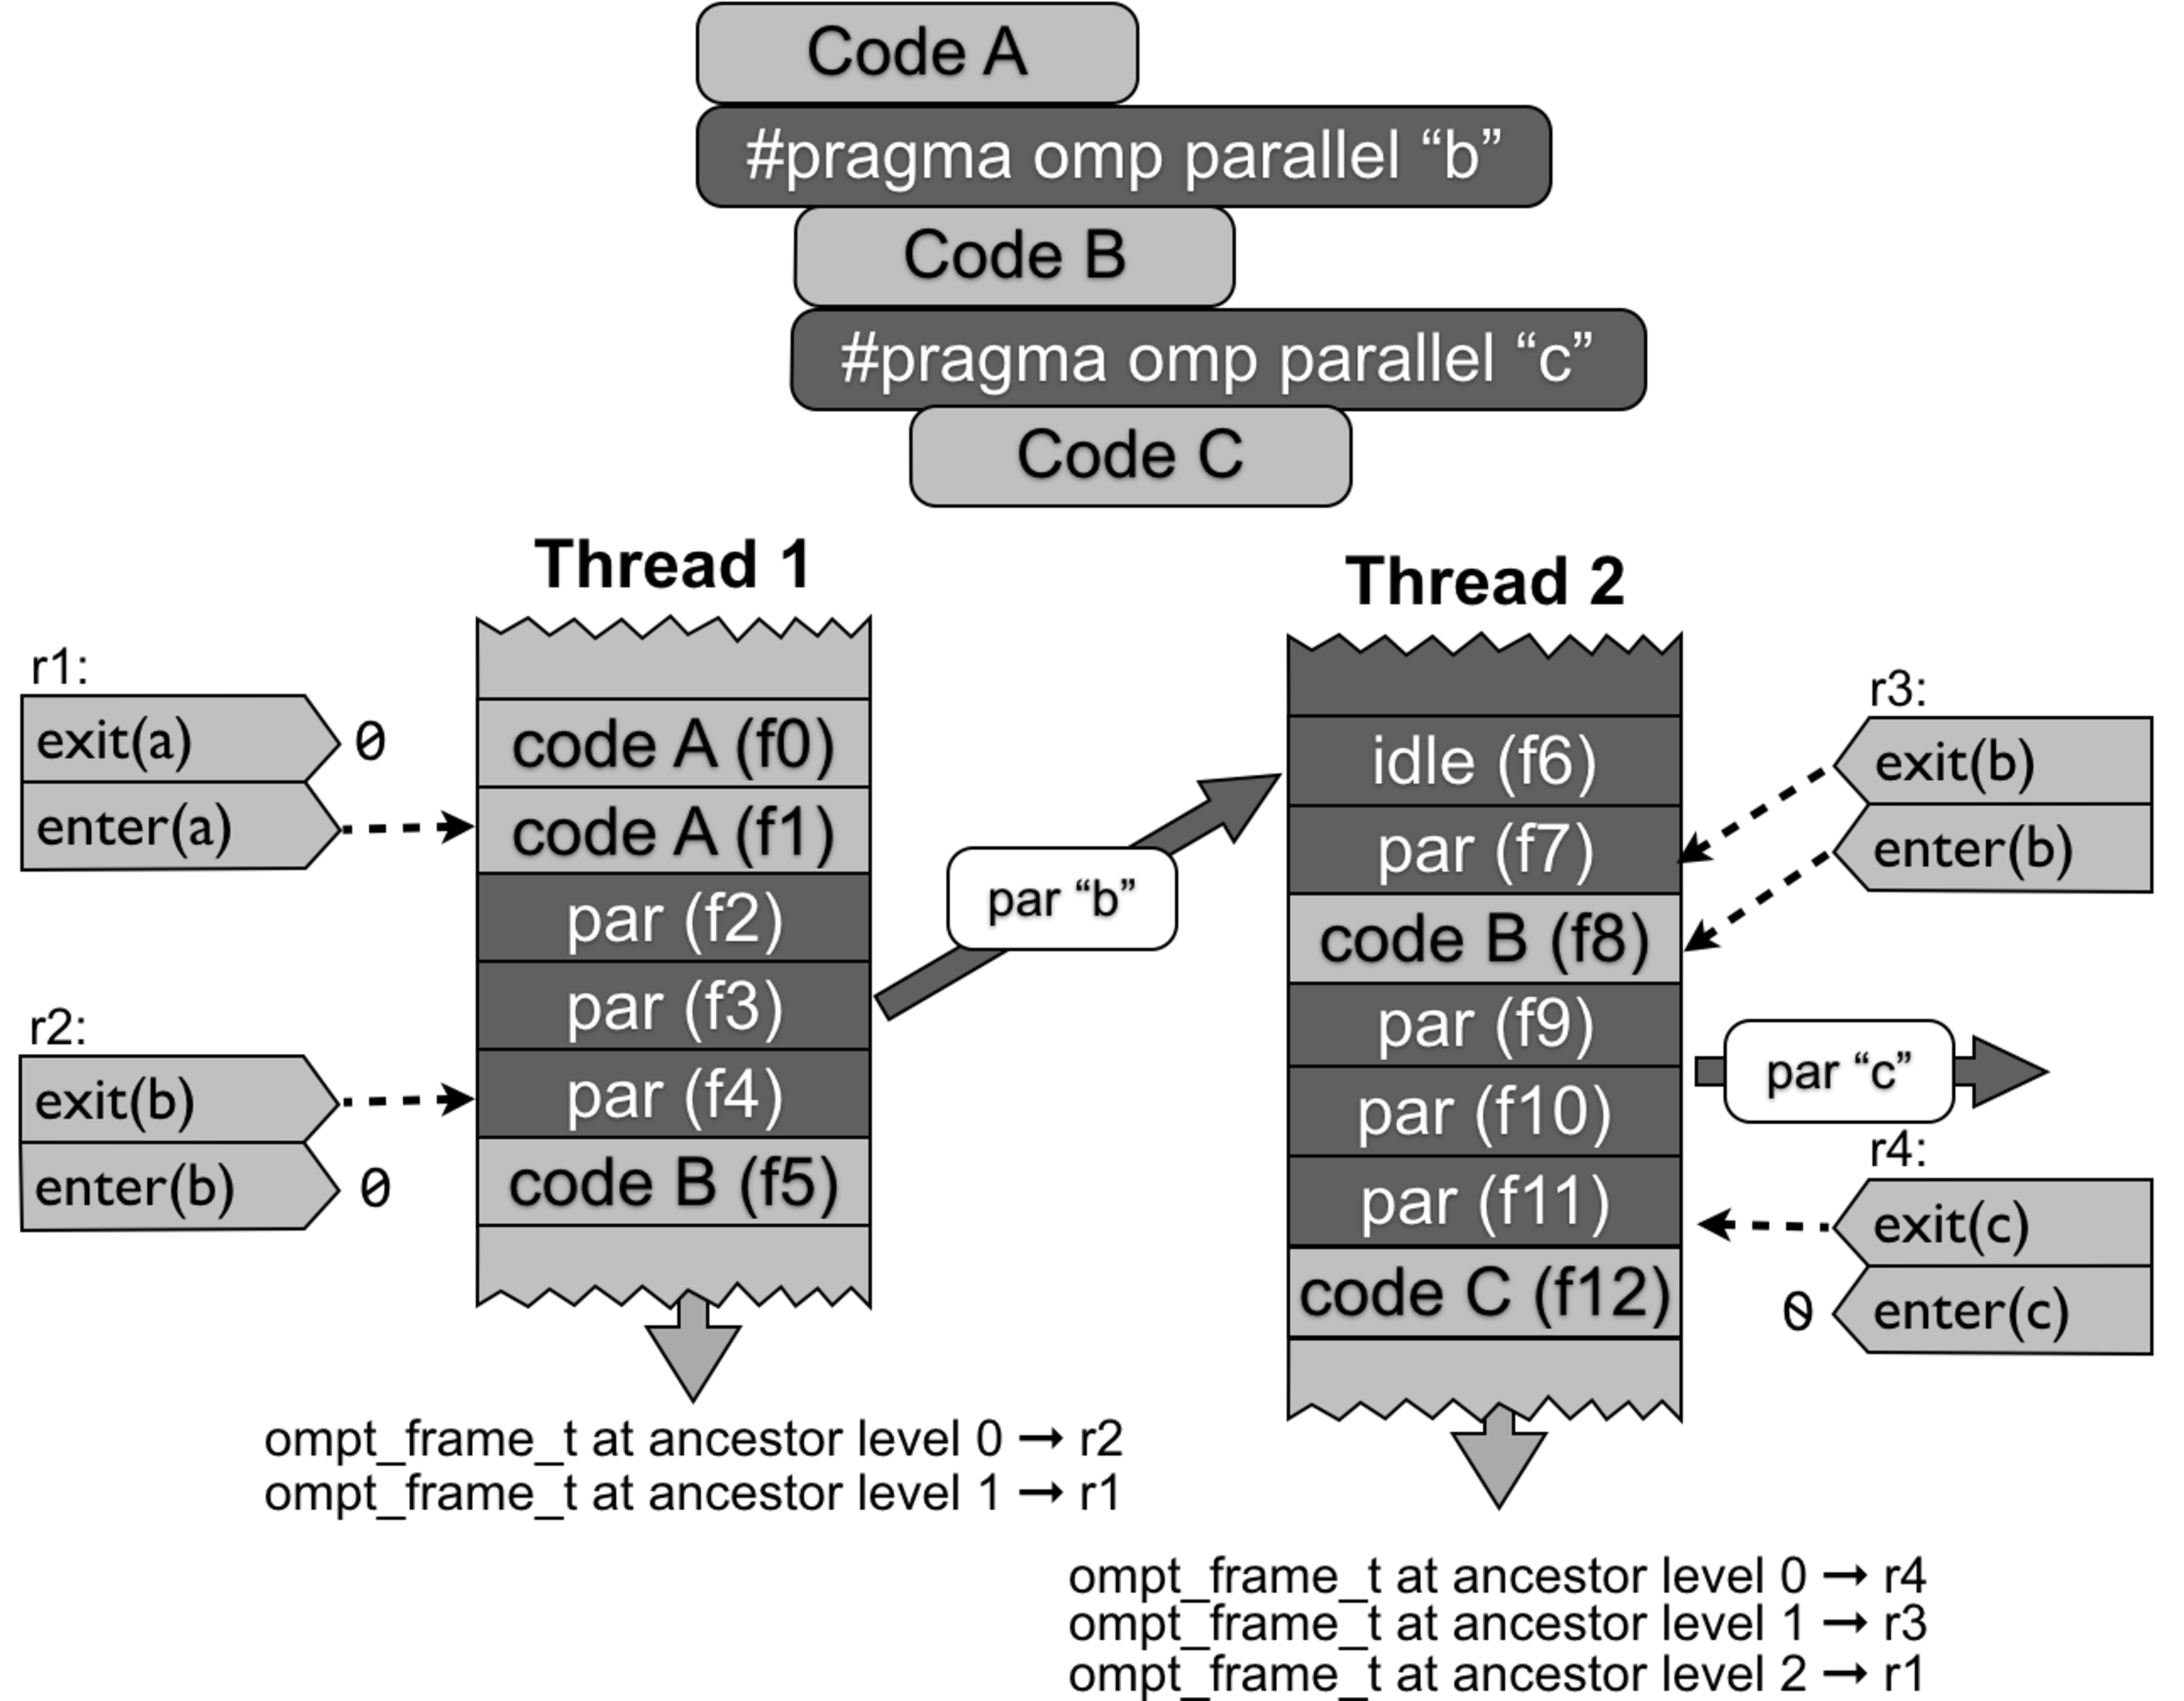
\includegraphics[width=4in]{callstack-cropped.pdf}
    \caption{Frame information.}
    \label{fig:frame}
\end{figure}

\noindent
Figure~\ref{fig:frame} illustrates a program executing a nested parallel region, where code A, B, and C represent, respectively, code associated with an initial task, outer-parallel, and inner-parallel regions.  Figure~\ref{fig:frame}  also depicts the stacks of two threads, where each new function call instantiates a new stack frame below the previous frames. When thread 1 encounters the outer-parallel region (parallel ``b"), it calls a routine in the OpenMP runtime to create a new parallel region. The OpenMP runtime sets the \code{enter\_frame} field in the \code{ompt\_frame\_t} for the initial task executing code A to  frame f1---the user frame in the initial task that calls the runtime. The  \code{ompt\_frame\_t} for the initial task is labeled  \code{r1} in Figure~\ref{fig:frame}. In this figure, three consecutive runtime system frames (labeled ``par'' with frame identifiers f2--f4) are on the stack. 
Before starting the implicit task for parallel region ``b" in thread 1, the runtime sets the \code{exit\_frame} in the implicit task's \code{ompt\_frame\_t}  (labeled \code{r2}) to f4. Execution of application code for parallel region ``b''  begins on thread 1  when the runtime system invokes application code B (frame f5) from frame f4. 

Let us focus now on thread 2, an OpenMP thread. Figure~\ref{fig:frame}  shows this worker executing  work for the outer-parallel region ``b."
On the OpenMP thread's stack is a runtime frame labeled ``idle,'' where the OpenMP thread waits for work. 
When work becomes available, the runtime system invokes a function to dispatch it. While dispatching parallel work might involve a chain of several calls, here we assume that the length of this chain is 1 (frame f7).  Before thread 2 exits the runtime to execute an implicit task for parallel region ``b,'' the runtime 
sets the \code{exit\_frame} field of the implicit task's \code{ompt\_frame\_t} (labeled \code{r3}) to frame f7. 
When thread 2 later encounters the inner-parallel region ``c,"  as execution returns to the runtime,  the runtime fills in the  \code{enter\_frame} field of the current task's \code{ompt\_frame\_t} (labeled \code{r3}) to frame f8---the frame that invoked the runtime. Before the task for parallel region ``c'' is invoked on thread 2, the runtime system sets the \code{exit\_frame} field  of the \code{ompt\_frame\_t} (labeled \code{r4}) for the implicit task for ``c'' 
to frame f11. Execution of application code for parallel region ``c''  begins on thread 2  when the runtime system invokes application code C (frame f12) from frame f11.


Below the stack for each thread in Figure~\ref{fig:frame}, the figure shows the \code{ompt\_frame\_t} information obtained by calls to \code{ompt\_get\_task\_info} made on each thread for the stack state shown. We show the ID of the \code{ompt\_frame\_t} record returned at each ancestor level. Note that thread 2 has task frame information for three levels of tasks, whereas thread 1 has only two.

\clearpage
{\color{red}
\section{Issues}
\begin{itemize}
\item distribute (fix all of the implications)
\item teams?
\end{itemize}
}

\end{document}
